\documentclass[12pt, a4paper, oneside]{report}             
\usepackage[czech]{babel}
\usepackage[utf8]{inputenc}  
\usepackage{graphicx} % balíček pro vkládání RASTROVÝCH grafických souborů (PNG apod.)
%\usepackage{epsfig} % balíčky pro vkládání VEKTOROVÝCH grafických souborů typu EPS
%\usepackage{float} % rozšířené možnosti umístění obrázků
%\usepackage{caption} % pro popisky obrázků, tabulek atd.
%\usepackage{tabularx} % rozšířené možnosti tabulek
%\usepackage{tabu} % jiný balík pro rozšířené možnosti tabulek
\usepackage{xcolor}
\usepackage{amsmath} % balíček pro pokročilou matematickou sazbu
\usepackage{pdfpages} % pro vkládání PDF souborů
%\usepackage{color} % pro možnost barevného textu
%\usepackage{fancybox} % umožňuje pokročilé rámečkování
%\usepackage{index} % nutno použít v případě tvorby rejstříku balíčkem makeindex
%\newindex{default}{idx}{ind}{Rejstřík} % zavádí rejstřík v případě použití balíku index
\usepackage{longtable}
\usepackage{array}
\usepackage[formats]{listings}  % Balíček pro sazbu zdrojových textů


\usepackage{anysize}
\marginsize{3.5cm}{1.5cm}{2.5cm}{3cm} % Nastavení okrajů (volitelné)

\usepackage{titlesec}  %přetypuje nadpisy všech úrovní na bezpatkové, tučné a dané velikosti

\titleformat{\chapter}[hang]{\sffamily\fontsize{16pt}{20pt}\bfseries}{\thechapter}{1em}{}
\titlespacing*{\chapter}{0pt}{20pt}{10pt}
\titleformat{\section}[hang]{\sffamily\fontsize{14pt}{16pt}\bfseries}{\thesection}{1em}{}
\titlespacing*{\section}{0pt}{20pt}{10pt}
\titleformat{\subsection}[hang]{\sffamily\fontsize{14pt}{18pt}\bfseries}{\thesubsection}{1em}{}
\titlespacing*{\subsection}{0pt}{20pt}{10pt}
\titleformat{\subsubsection}[hang]{\sffamily\fontsize{14pt}{18pt}\bfseries}{\thesubsubsection}{1em}{}
\titlespacing*{\subsubsection}{0pt}{20pt}{10pt}

\usepackage{setspace}
\setstretch{1.3} % Nastaví 1,3násobné řádkování

\frenchspacing % za větou bude mezislovní mezera (v anglických textech je mezera za větou delší)
\widowpenalty=1000 % "síla" zákazu vdov (= jeden řádek odstavce na konci stránky)
\clubpenalty=1000 % "síla" zákazu sirotků (= jeden řádek/slovo odstavce samostatně na začátku stránky)
\brokenpenalty=1000 % "síla" zákazu zlomu stránky za řádkem, který má na konci rozdělené slovo

\pagenumbering{arabic} % číslování stránek arabskými číslicemi
\usepackage{fancyhdr} % Načte balíček pro pokročilé úpravy záhlaví a zápatí.
\pagestyle{fancy} % Nastavení stylu stránek na 'fancy'
\fancyhf{} % Vymazání aktuálního nastavení záhlaví a zápatí
\fancyfoot[R]{\thepage} % Nastavení čísel stránek vpravo dole (R - right)
\renewcommand{\headrulewidth}{0pt}
\renewcommand{\footrulewidth}{0pt}
\fancypagestyle{plain}{%
  \fancyhf{}
  \fancyfoot[R]{\thepage}
  \renewcommand{\headrulewidth}{0pt}
  \renewcommand{\footrulewidth}{0pt}
}
\parindent=0pt % odsazení 1. řádku odstavce
\parskip=12pt   % mezera mezi odstavci
\usepackage[breaklinks=true,hypertexnames=false]{hyperref}  % Balíček 'hyperref' pro sazbu hypertextových odkazů. Hypertextové odkazy mohou obsahovat zalomení řádku. Názvy hypertext. odkazů budou tvořeny nezávisle na názvech TeXu.
\hypersetup{ % popisky v pdf souboru
  pdftitle={Název studentské práce},    	% Pole 'Document Title'
  pdfauthor={Autor studentské práce},   	% Pole 'Author'
  pdfsubject={Typ práce}, 						  	% Pole 'Subject'
  pdfkeywords={Klíčová slova}           	% Pole 'Keywords'
}

%%%%%%%%%%%%%%%%%%%%%%%%%%%%%%%%%%%%%%%%%%%%%%%%%%%%%%%%%%%%%%%%%%%%%%%
%%%%%%%%%%%       Začátek dokumentu               %%%%%%%%%%%%%%%%%%%%%
%%%%%%%%%%%%%%%%%%%%%%%%%%%%%%%%%%%%%%%%%%%%%%%%%%%%%%%%%%%%%%%%%%%%%%%
\begin{document}
\thispagestyle{empty} %vypnutí číslování stránek


%% TITULNÍ STRANA %%%%%%%%%%%%%%%%%%%%%%%%%%%%%%%%%%%%%%%%%%%%%%%%%%%%%%%%%%%%%%
\begin{center}
  \begin{minipage}{3cm}
    
\includegraphics[width=2.86cm]{Logo.png}
  \end{minipage}
  \hfill
  \begin{minipage}{0.7\textwidth}
    \centering
    {\Large Vyšší odborná škola\\
    a Střední průmyslová škola elektrotechnická\\
    Plzeň, Koterovská 85\\ }
  \end{minipage}
  
  \vspace{2cm}
  %% VYBERTE TYP PRÁCE %%%%%%%%%%%%%%%%%%%%%%%%%%
  %%{\Large \textbf{DLOUHODOBÁ MATURITNÍ PRÁCE S~OBHAJOBOU}\\ }
  {\Large \textbf{ROČNÍKOVÁ PRÁCE}\\ }
  %%%%%%%%%%%%%%%%%%%%%%%%%%%%%%%%%%%%%%%%%%%%%%%
  
  \vspace{2.5cm}
  {\large Téma: \\ }
  \vspace{0.25cm}
  %% PŘEPIŠTE NÁZEV PRÁCE %%%%%%%%%%%%%%%%%%%%%%%%%%%
  {\LARGE \textbf{Fotaoparát - Systém pro obsluhu kamery}}  
  %%%%%%%%%%%%%%%%%%%%%%%%%%%%%%%%%%%
  
  \vfill
\end{center}
\begin{tabular}{{p{4.5cm} p{12cm}}}
  {\Large \textbf{Autor práce:}} & \Large{Vít Hovorka}\\
  {\Large \textbf{Třída:}} & \Large{3.L}\\ 
  {\Large \textbf{Vedoucí práce:}} & \Large{Jiří Švihla} \\ 
  {\Large \textbf{Dne:}} & \Large{30.4.2026} \\ 
  {\Large \textbf{Hodnocení:}} &  \\ 
\end{tabular}
%% Vložení zadání %%%%%%%%%%%%%%%%%%%%%%%%%%%%%%%%%%%%%%%%%%%%%%%%%%%%%%%%%%%%
\newpage
\thispagestyle{empty}
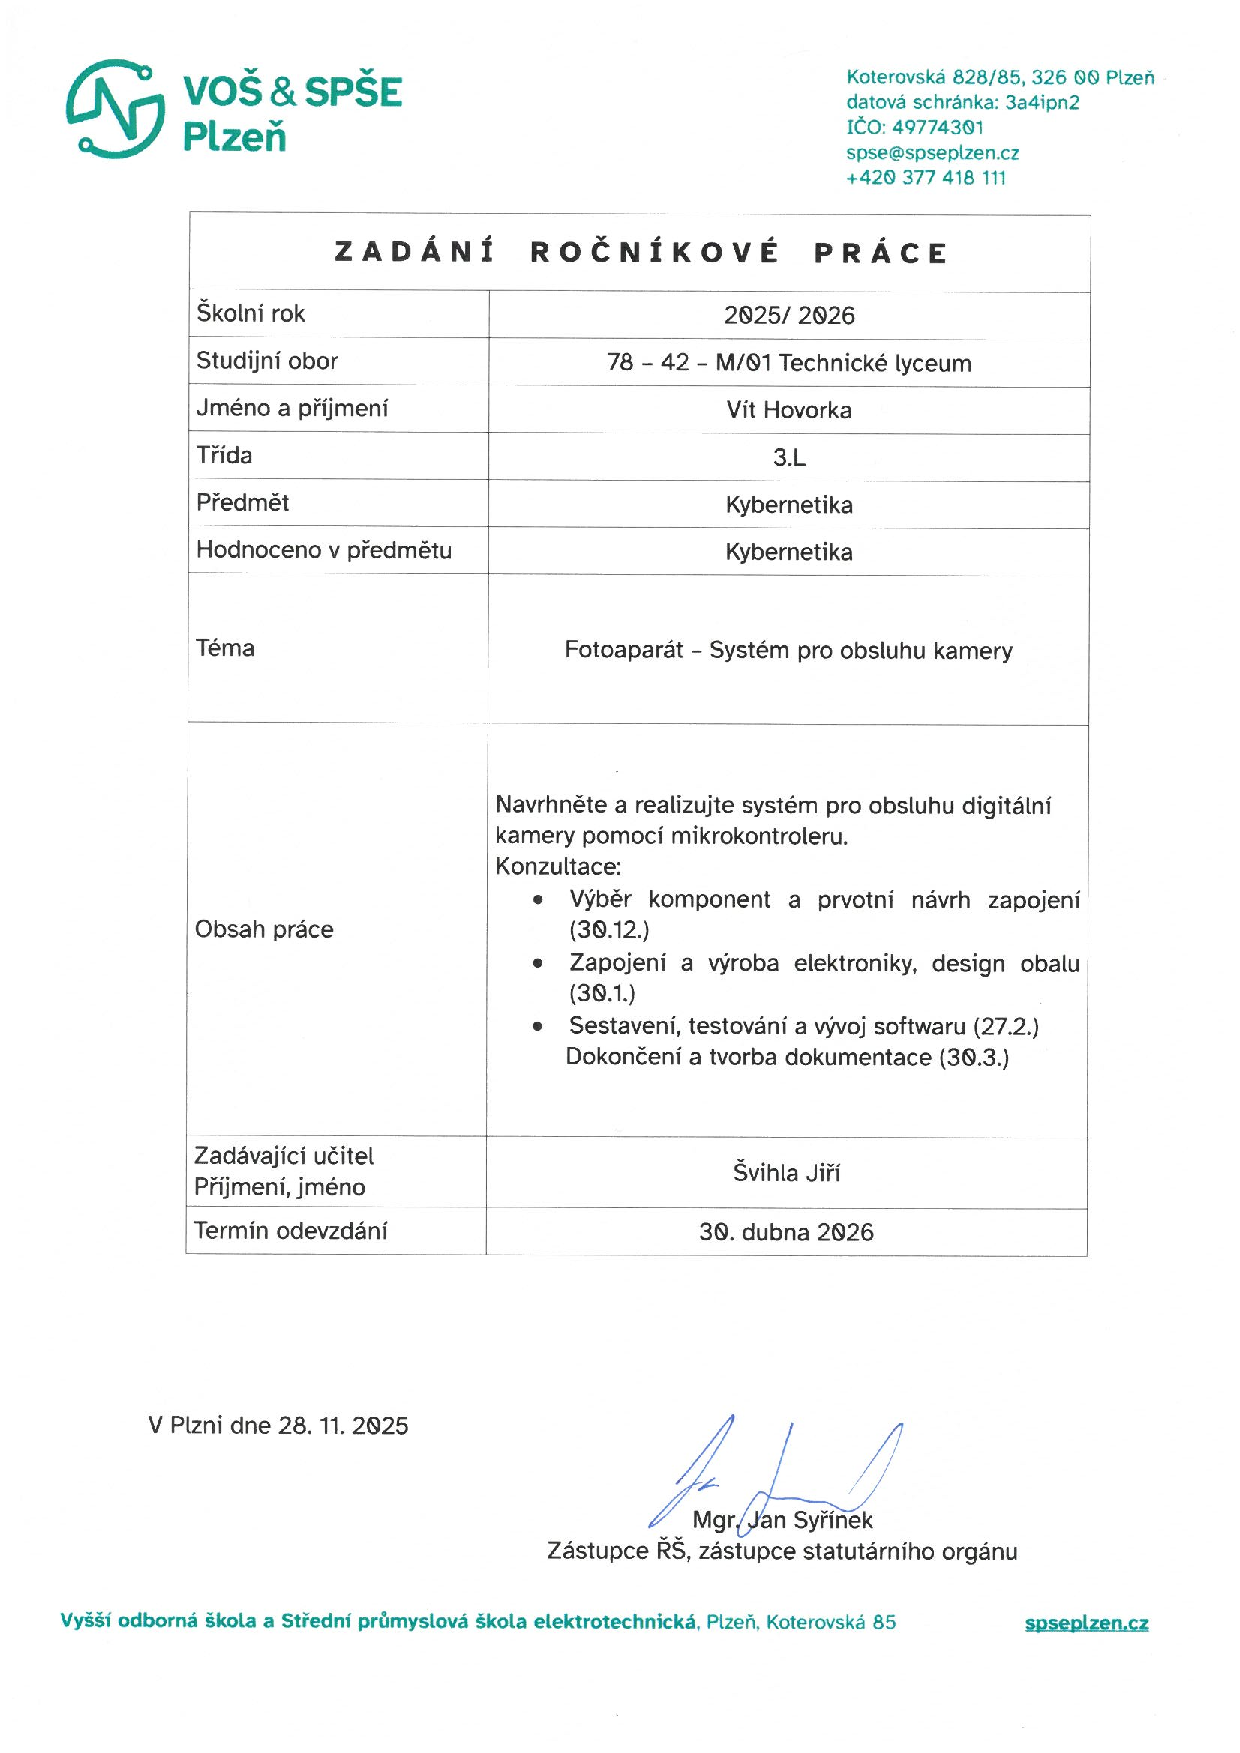
\includepdf{pdf/Zadani-Hovorka.pdf}% název souboru nesmí obsahovat mezery!
%% NEBO lze vytvořit prázdný list příkazem ze šablony

%\newpage   % při dvojstranném tisku se přidá prázdná stránka


%%%%%%%%%%%% Anotace a poděkování %%%%%%%%%%%%%%%%%%%%%%%%%%%%%%%%%%%%%%%%%%%%%%
\newpage
\chapter*{Anotace} \indent
\thispagestyle{empty}

Cílem této ročníkové práce je vytvořit systém pro obsluhu mikrokontrolérové kamery, za pomoci mikrokontroléru \texttt{ESP32-P4}. Tím se rozumí od výběru součástek a návrhu PCB až po naprogramování vlastního operačního softwaru. 
\vfill

Prohlašuji, že jsem tuto práci vypracoval samostatně a použil literárních pramenů a~\mbox{informací}, které cituji a uvádím v seznamu použité literatury a zdrojů informací.

Prohlašuji, že jsem nástroje UI využil v souladu s principy akademické integrity a že na využití těchto nástrojů v práci vhodným způsobem odkazuji.

Souhlasím s využitím mé práce učiteli VOŠ a SPŠE Plzeň k výuce.

\vspace{1cm}

V Plzni dne 30. 4. 2026 \hfill Podpis: ..........................

%%%%%%%%%%%% Obsah práce ... je generován AUTOMATICKY %%%%%%%%%%%%
\newpage
\tableofcontents
\thispagestyle{empty}

%%%%%%%%%%%% Seznam zkratek %%%%%%%%%%%%%%%%%%%%%%%%%%%%%%%%%%%%%%%%%%%%%%
\newpage
\chapter*{Seznam zkratek}
\addcontentsline{toc}{chapter}{Seznam zkratek}
\begingroup
\setlength{\tabcolsep}{6pt}
\renewcommand{\arraystretch}{1.4}
\begin{longtable}{>{\raggedright\arraybackslash}p{2.6cm} >{\raggedright\arraybackslash}p{6.3cm} >{\raggedright\arraybackslash}p{5.2cm}}

\textbf{Zkratka} & \textbf{Anglicky} & \textbf{Česky} \\
\endfirsthead
\textbf{Zkratka} & \textbf{Anglicky} & \textbf{Česky} \\
\endhead
ADC & Analog-to-digital converter & analogově-digitální převodník \\
AF & Autofocus & automatické ostření \\
CSI & Camera Serial Interface & kamerové sériové rozhraní \\
DRC & Design Rules Check & kontrola pravidel návrhu \\
DSI & Display Serial Interface & zobrazovací sériové rozhraní \\
DTR & Double Transfer Rate & přenos na obou hranách hodinového signálu \\
ERC & Electrical Rules Check & kontrola elektrických pravidel \\
ESP-IDF & Espressif IoT Development Framework & vývojový rámec pro čipy ESP od společnosti Espressif \\
ESD & Electrostatic discharge & elektrostatický výboj \\
GPIO & General-purpose input/output & univerzální vstup/výstup \\
HP & High Power & vysoký výkon\\
I2C & Inter-Integrated Circuit & dvouvodičová sériová sběrnice \\
NOR & NOR flash & typ nevolatilní flash paměti \\
ISO & International Organization for Standardization & citlivost podle fotografické terminologie \\
LP & Low Power & Nízký výkon\\
MILC & Mirrorless interchangeable-lens camera & bezzrcadlový fotoaparát s výměnnými objektivy \\
MCU & Microcontroller unit & mikrokontrolér \\
MIPI & Mobile Industry Processor Interface & standard mobilního rozhraní pro periférie \\
PCB & Printed circuit board & plošný spoj \\
QSPI & Quad Serial Peripheral Interface & čtyřlinkové sériové periferní rozhraní \\
SD & Secure Digital & paměťová karta Secure Digital \\
SPI & Serial Peripheral Interface & sériové periferní rozhraní \\
USB & Universal Serial Bus & univerzální sériová sběrnice \\
\caption{Seznam zkratek}
\end{longtable}
\endgroup

%--------------------------------------------------------
%|         Zde začíná SAMOTNÁ PRÁCE (text)              |
%--------------------------------------------------------
\newpage

\chapter*{Úvod}
\addcontentsline{toc}{chapter}{Úvod}
Už asi dva roky se pokouším být aktivním fotografem, s tím že jsem začínal na analogovém fotoaparátu a snažil se naučit souvislosti mezi hodnotami expozičního času, clony a ISO. Vždy mě bavilo zkoumat do hloubky jak a proč takové věci fungují a hledat si svou vlastní „cestu trním"~kde metodou pokus omyl šlechtím své dovednosti. Proto mi sestavení svého vlastního fotoaparátu přišlo jako dobrá cesta jak naučit nejen elektrotechniku a programovaní, ale i jak poznat technologii digitální fotografie do hloubky.

\chapter{Cíle a požadavky}
\section{Požadavky na mechanické konstrukční řešení}
Tento projekt by měl v ideálním případě alespoň připomínat MILC kameru. Výrobek, dále označovaný jako fotaoparát, by měl být tedy:
\begin{itemize}
    \item svými rozměry a tvarem podobný dnešním digitálním fotoaparátům,
    \item jednoduše nositelný a ovladatelný,
    \item kompatibilní s objektivy řady Canon EF. Toto rozhodnutí má jak objektivní tak i subjektivní opodstatnění. Subjektivní rovinou zde je fakt že už několika disponuji. V objektivní rovině je fakt že komunikační protokoly jsou už komunitou zmapovány (Magic Lantern\footnote{Magic Lantern firmware, dostupné z: https://www.magiclantern.fm}).
\end{itemize}
\section{Požadavky na elektrotechnické řešení}
Součástí vývoje projektu je i návrh základní desky pro mikročip \texttt{ESP32-P4} a jeho periférií. Základní deska tedy:
\begin{itemize}
    \item bude mít na starost napájení jak hlavního čipu, tak veškerých periférií. Napájení bude zajištěno jedním akumulátorem,
    \item obstará všechny konektory pro zapojení periférií. Bude tedy možné případné periferie vyměnit za lepší za předpokladu kompatibility z hlediska počtu vývodů (pinů) na konektoru a prostoru v těle Fotaoparátu,
    \item bude jednoduše programovatelná pomocí USB-C vstupu. Fotaoparát bude open-source výrobek podporující a vyzývající k úpravám podle uživatele, kde open-source znamená výrobek s veřejně dostupným zdrojovým kódem,
    \item bude navrhována s ohledem na elektromagnetické rušení signálů a možnosti ztráty dat kvůli délkové asymetrii cest a design se tedy bude snažit toto rušení a ztrátu minimalizovat.
    \item bude navrhována s ohledem na prostor a konstrukční provedení těla fotaoparátu. Bude tedy dostatečně skladná a vývody na periferie budou vhodně umístěny.
\end{itemize}
\section{Požadavky na softwarové řešení}
Výrobek bude nakonec oživen firmwarem vlastní výroby. Software bude mít pevně dané funkce jako např. nastavení hodnot ISO, clony a rychlosti závěrky. Zároveň by měl mít jednoduše přizpůsobitelné uživatelské rozhraní a možnost přidávat další uživatelské funkce.
\chapter{Použité nástroje}
\section{KiCAD 9.0}
Pro návrh samotné základní desky Fotaoparátu jsem zvolil software KiCAD 9.0. Jedná se o open-source software určený pro návrh elektronických schémat a plošných spojů. Samotný program totiž ukrývá tři hlavní podprogramy: Schematic editor, PCB editor a Gerber viewer.

Schematic editor umožňuje uživateli nakreslit elektrické schéma a dokonce i do jisté míry simulovat jednoduché elektrické obvody. Dále KiCAD hned po instalaci disponuje velmi rozmanitou knihovnou součástek, pouzder a datasheetů (technická dokumentace jednotlivých součástek). Stačí si tedy součástky vybrat, pomocí nástroje „kreslit vodiče" je propojit, nebo pomocí nástroje „označení sítě" jim přiřadit stejnou síť. Je zde také možnost využít nástroj ERC (electrical rules check - kontrola elektrických pravidel), ten slouží k odhalení chyb v zapojení vývodů.
\begin{figure}
    \centering
    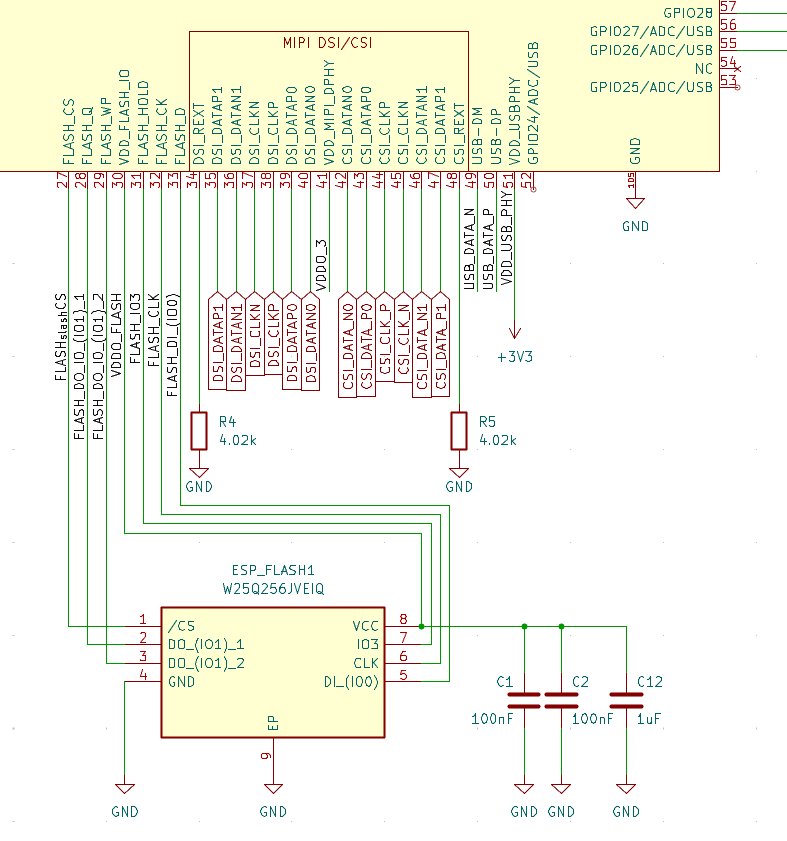
\includegraphics[width=0.5\linewidth]{pictures/eeschema.png}
    \caption{Ukázka programu schematic editor \textit{Zdroj: [vlastní]}}
    \label{fig:schematicsmrdito}
\end{figure}

PCB editor slouží k přímému návrhu plošného spoje. Obvyklý postup při práci s KiCADem je nakreslení elektronického schématu, přiřazení pouzder, načtení těchto dat do PCB editoru a zde rozmístit součástky a routovat cesty spojů. Disponuje také možností nastavení konstrukčních vlastností desky (počet vrstev, tloušťka jednotlivých vrstev, základní tloušťka spojů, velikost prokovených otvorů, minimální požadovaná vzdálenost mezi cestami...).
Pro kontrolu designových chyb na desce pak slouží nástroj DRC (design rules check - kontrola pravidel designu).
\begin{figure}
    \centering
    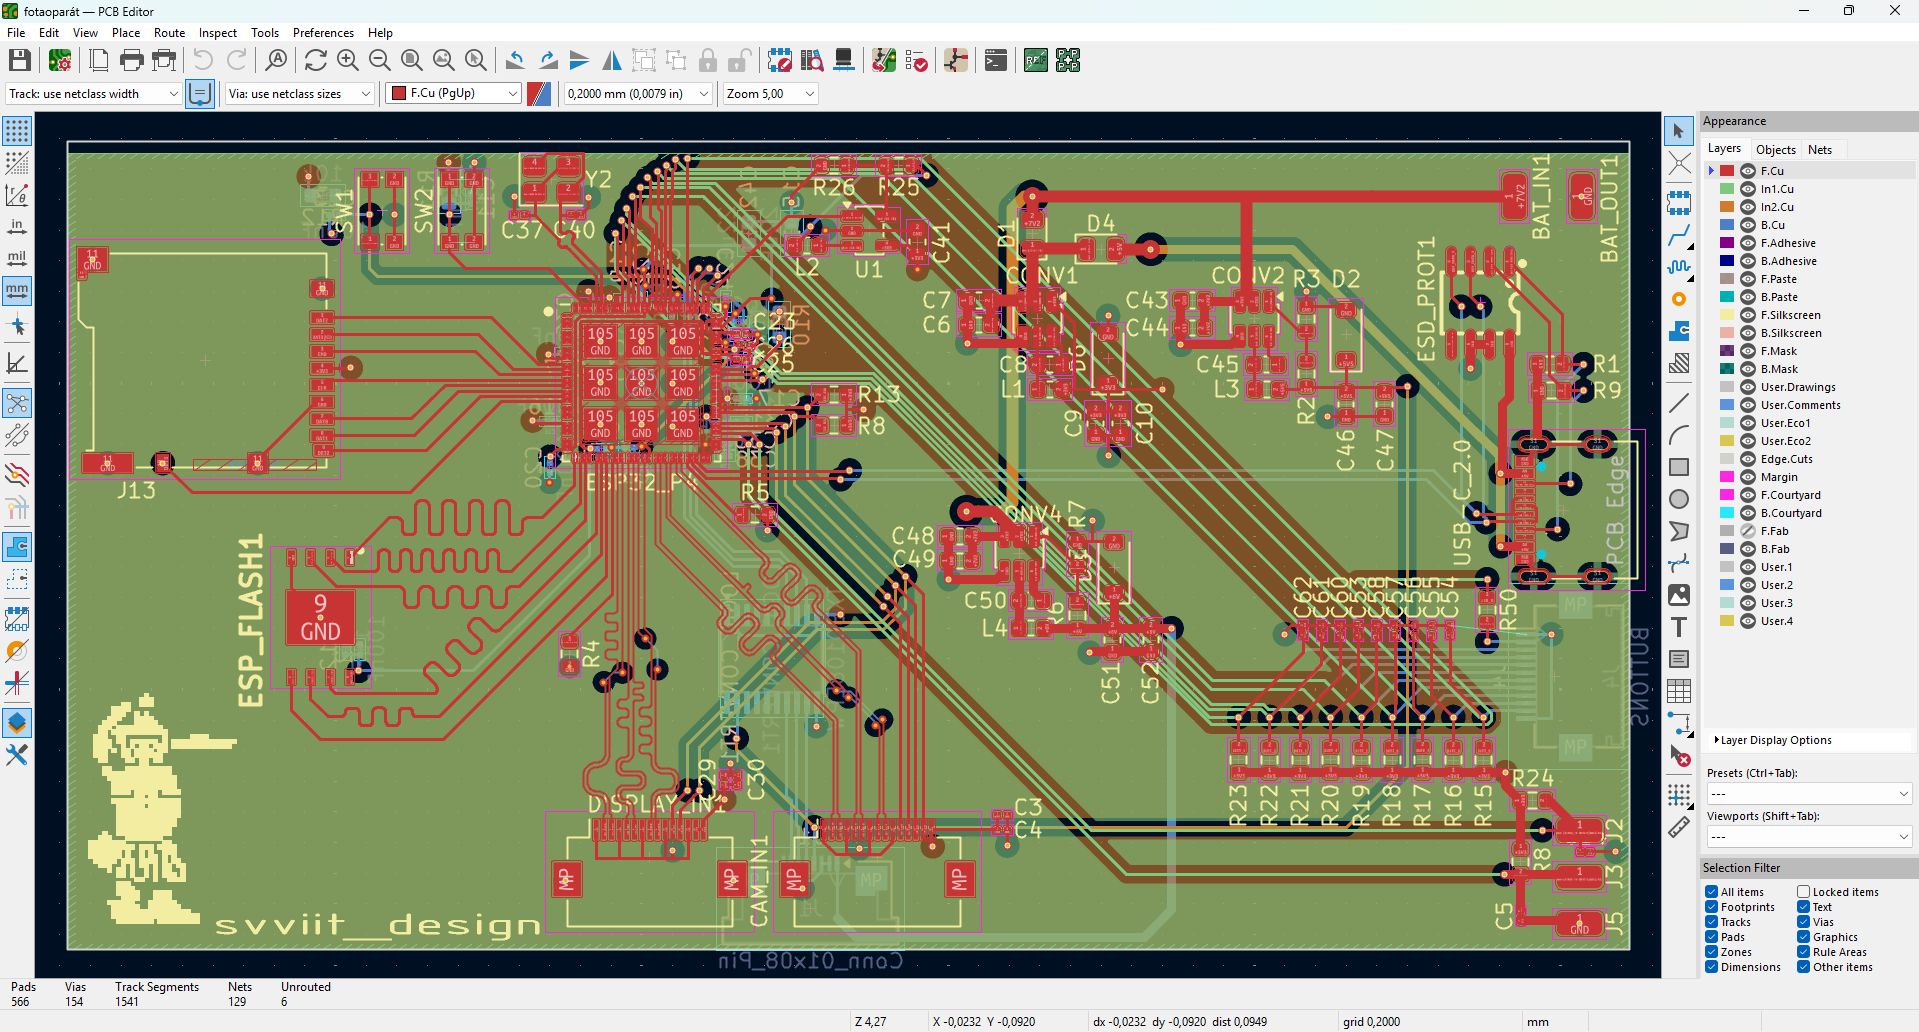
\includegraphics[width=1\linewidth]{pictures/pcbeditor.png}
    \caption{Ukázka programu PCB editor \textit{Zdroj: [vlastní]}}
    \label{fig:pcbsmrdito}
\end{figure}

Jako poslední podstatná část programu KiCAD je gerber viewer. Ten slouží k exportu geberových dat pro výrobu desky.

\section{Visual Studio Code}
Visual Studio Code (zkráceně VS Code nebo VS) je bezplatné moderní vývojové prostředí. Díky velkému množství rozšíření, která lze instalovat přímo v programu, a podpoře hlavních operačních systémů (Windows, Linux a macOS) si získalo značnou oblibu mezi programátory.

\begin{figure}
    \centering
    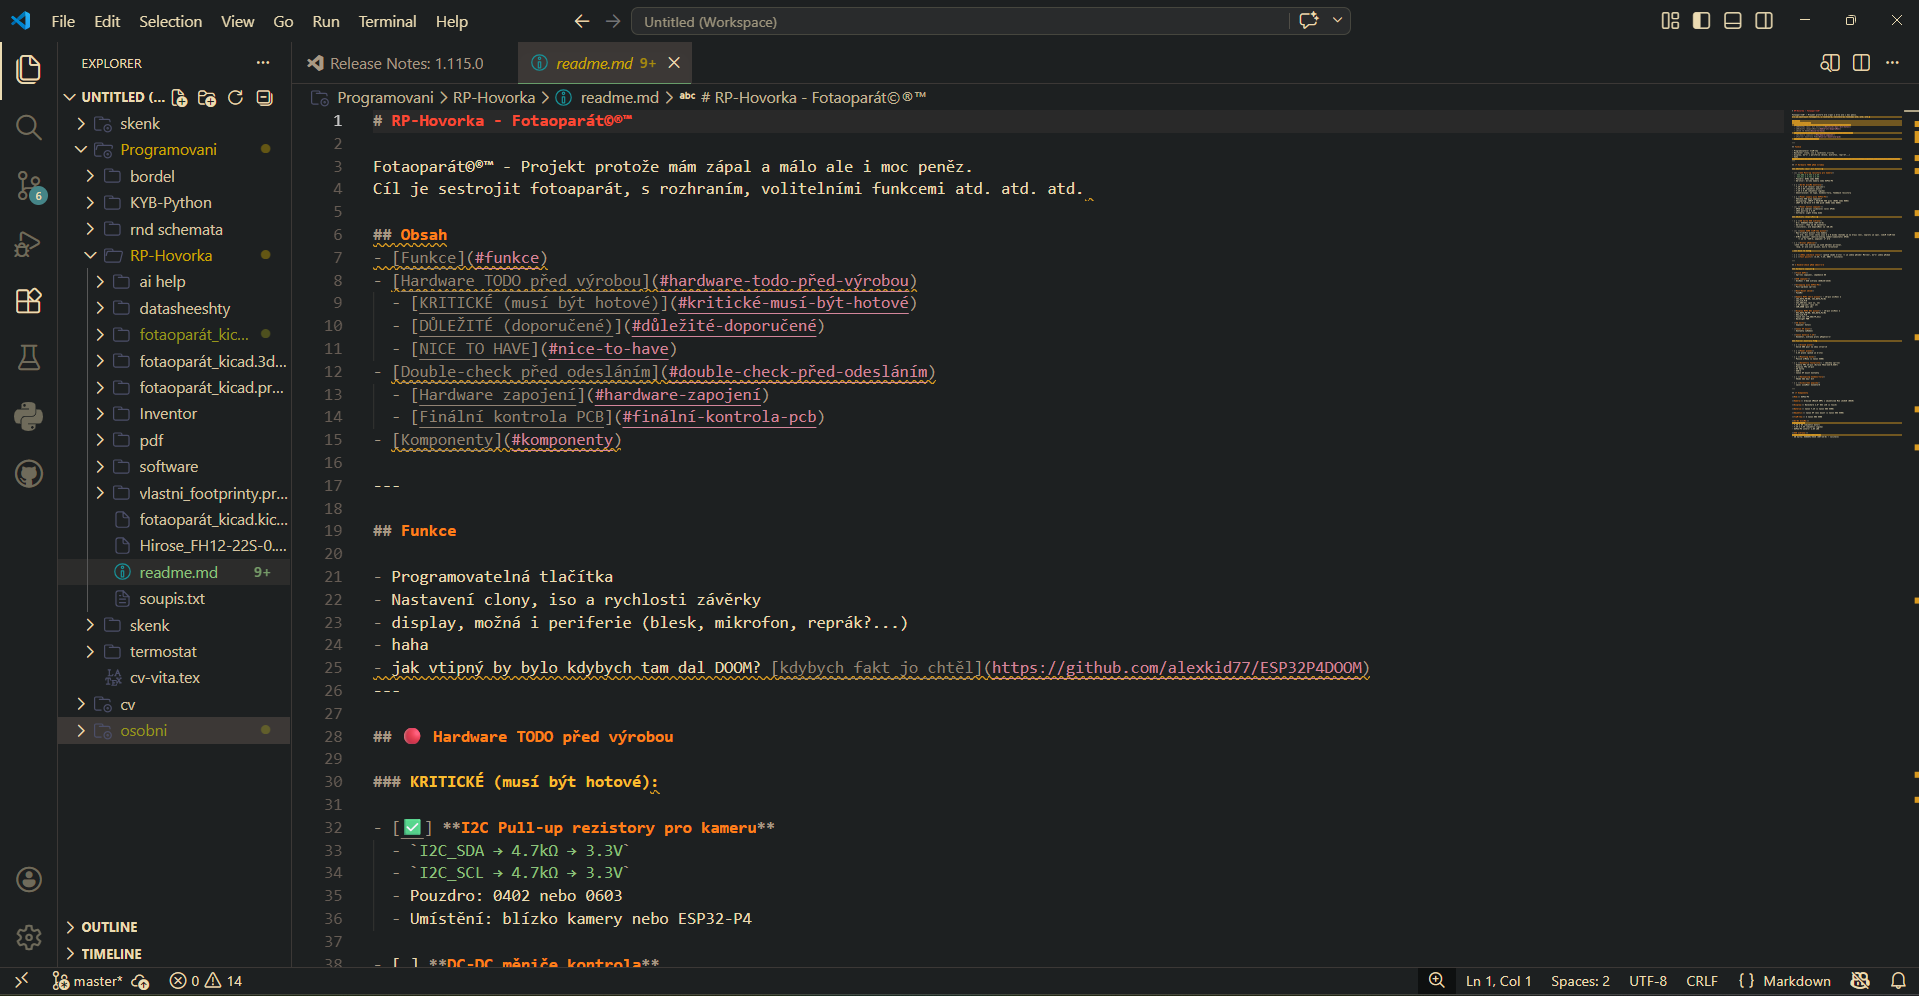
\includegraphics[width=1\linewidth]{pictures/vsko.png}
    \caption{Ukázka programu Visual Studio Code \textit{[Zdroj: Vlastní]}}
    \label{fig:vsko}
\end{figure}

Mezi jeho hlavní funkce patří podpora verzovacích systémů jako např. Git, zvýraznění syntaxe (např. závorkové páry), našeptávání kódu, integrovaný terminál a debugger.

V mé práci jsem VS používal zejména pro jednoduché commitování. Dále jsem v něm používal umělou inteligenci pomocí které jsem napsal část firmwaru. 
\chapter{Vybrané komponenty}
\section{MCU}
Kvůli vysoké výpočetní náročnosti zpracování dat, která představuje jediný snímek o rozlišení 8 Mpx, bylo nutné zvolit jeden z nejvýkonnějších mikrokontrolérů dostupných v době realizace projektu — \texttt{ESP32-P4}. Jedná se o moderní MCU navržené s důrazem na vysoký výpočetní výkon, multimediální zpracování a efektivní práci s periferiemi\cite{esp32p4_ds}.

\texttt{ESP32-P4} je vybaven vícejádrovou architekturou, která umožňuje paralelní zpracování úloh. V tomto MCU se nacházzejí dva procesory -- jednojádrový a pomalejší LP a dvoujádrový rychlejší HP. Oba procesory jsou postaveny na 32-bitové architektuře. 

Low power procesor má nejvyšší rychlost taktu 40 MHz. Je narvžený pro zastoupení HP obvodů při sleep režimu, jelikož i při deep--sleep reimu je tento procesor a jeho pamět aktivní. Zároveň má však přístup i do HP paměti. 

High Power procesor má nejvyšší rychlost taktu 360 Mhz Dále disponuje hardwarovou akcelerací pro vybrané operace. Jeho paměti zahrnují:
\begin{itemize}
    \item 16 MB SRAM
    \item 128 kB ROM pro HP obvody
    \item 768 kB HP L2mem
    \item 16 kB ROM pro LP obvody
    \item 8 kB systémové SPM
    \item Více vyoskorychlostními externími paměťovými rozhraními
    \item Dvouúrovňovou vysokorychlotní cache
\end{itemize} 

Čip také zahruje podporou vysokorychlostních rozhraní, jako např. CSI, DSI a QSPI, která umožňují efektivní přenos velkého množství dat.

\section{Flash paměť}
Další důležitou součástí návrhu je externí flash paměť. Mikrokontrolér \texttt{ESP32-P4} totiž nedisponuje dostatečně velkou interní pamětí pro uložení uživatelského kódu, a proto je nutné využít externí úložiště.

V tomto projektu byla zvolena paměť \texttt{W25Q256JV-DTR} od společnosti Winbond. Jedná se o sériovou NOR flash paměť s kapacitou 256 Mbit (32 MB), která slouží pro ukládání firmwaru, konfiguračních dat a případně i dočasných obrazových dat.

Paměť komunikuje s mikrokontrolérem prostřednictvím rozhraní SPI, respektive jeho rozšířené varianty QSPI, která umožňuje paralelní přenos dat po více datových linkách. Díky tomu lze dosáhnout výrazně vyšších přenosových rychlostí oproti standardnímu SPI, což je zásadní zejména při práci s obrazovými snímky.

Označení DTR (Double Transfer Rate) znamená, že data jsou přenášena na obou hranách hodinového signálu, čímž dochází k efektivnímu zdvojnásobení propustnosti bez nutnosti zvyšování pracovní frekvence. Tato vlastnost přispívá ke zvýšení celkového výkonu systému při čtení i zápisu dat.

Paměť je organizována do sektorů, což umožňuje efektivní mazání a zápis po blocích. Zároveň podporuje mechanismy ochrany vybraných oblastí proti zápisu, což je výhodné například pro zabezpečení kritických částí firmwaru.
\section{Kamerový modul}
Další klíčovou komponentou je kamerový modul Arducam \texttt{IMX219} s rozlišením 8 Mpx. Tento modul byl zvolen nejen s ohledem na příznivý poměr ceny a výkonu, ale také díky své kompatibilitě a vhodnosti pro použití s mikrokontrolérem \texttt{ESP32-P4}.

Zde je klíčové rozhraní DSI/CSI, které umožňuje vysokorychlostní přenos obrazových dat mezi kamerovým modulem, případně displejem, a samotným mikrokontrolérem. Využití tohoto rozhraní je zásadní zejména kvůli vyšším přenosovým rychlostem. Pokud bychom zvolili jiný postup, vyžadovalo by to desítky GPIO pinů, které prostě na MCU nemáme, a navíc by to bylo velmi náročné na synchronizaci a zpracování dat.

Samotný snímač \texttt{IMX219} nabízí dostatečné rozlišení pro zamýšlenou aplikaci a zároveň podporuje různé režimy výstupu, což umožňuje optimalizovat kompromis mezi kvalitou obrazu a objemem přenášených dat. V jednoduchosti můžeme poté přímo ve Fotaoparátu nastavovat rozlišení výstupního snímku.

Výhodou modulu Arducam je také jeho široká podpora a dostupná dokumentace, což usnadňuje jeho integraci do návrhu jak na hardwarové, tak i softwarové úrovni.

\section{Display}
Pro zobrazovací jednotku jsem zvolil 2,8"~LCD modul od společnosti Waveshare, a to především díky jeho DSI rozhraní, které je podporováno mikrokontrolérem ESP32-P4. Toto rozhraní umožňuje efektivní a rychlou komunikaci mezi řídicí jednotkou a displejem.

Dalším důvodem výběru tohoto konkrétního displeje byla jeho kompatibilita s mechanickou konstrukcí zařízení. Pro zjednodušení návrhu jsem se rozhodl využít tělo a vybrané periferie fotoaparátu Canon 550D. Pro účely této kapitoly postačí uvést, že původní displej z modelu 550D není vhodné použít, jelikož k němu není veřejně dostupná dostatečná technická dokumentace. Zároveň má však velmi podobné rozměry jako zvolený Waveshare modul, což usnadňuje jeho náhradu bez nutnosti zásadních mechanických úprav.

\section{Konektor pro SD kartu}

Pro ukládání dat bude použit konektor pro SD kartu, což představuje standardní řešení úložiště u digitálních fotoaparátů. SD karty jsou kompaktní, široce rozšířené a snadno dostupné externí médium, které nabízí dostatečné přenosové rychlosti pro zamýšlenou aplikaci. Oproti tomu běžné USB flash disky nejsou pro tento typ zařízení tak vhodné, a to jak z hlediska rozměrů, tak i způsobu připojení.

Alternativou by mohlo být použití paměťových karet typu CompactFlash. Tyto karty sice teoreticky dosahují vyšších přenosových rychlostí, mimo jiné díky většímu počtu pinů, avšak jejich nevýhodou je vyšší pořizovací cena. Dalším omezením je skutečnost, že konektory pro CompactFlash karty jsou v současnosti obtížně dostupné a často vyžadují použití redukce. Z těchto důvodů nebylo toto řešení dále uvažováno.
\section{Konektor pro komunikaci s počítačem.}
Pro nahrávání firmwaru je na desce navržen USB-C konektor, který slouží nejen pro samotné programování mikrokontroléru, ale také pro jeho napájení během vývoje a testování. Toto řešení výrazně zjednodušuje proces nasazení firmwaru, protože není nutné využívat externí programátor.
\chapter{Podrobné zapojení na desce}
\section{MCU}
Středem celého návrhu je mikrokontrolér ESP32-P4, osazený jako hlavní výpočetní a řídicí prvek.
\begin{figure}
    \centering
    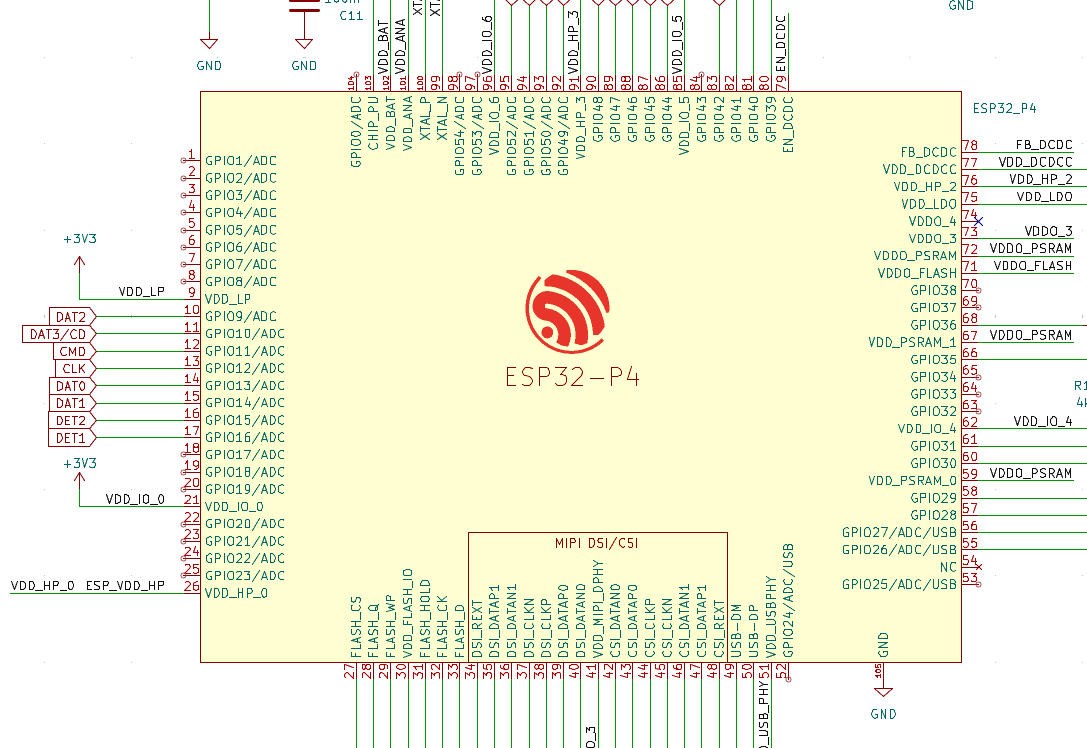
\includegraphics[width=0.7\linewidth]{pictures/esp32-p4.png}
    \caption{ESP32-P4 v eschématu \textit{[Zdroj: Vlastní]}}
    \label{fig:esp32p4}
\end{figure}

Sám o sobě ale být použit nemůže. Pro jeho ideální funkci je potřeba externí flash pamět, externí krystal a externí buck converter na 1,1 V pro napájení high power pinů.

\subsection{Napájení interní SRAM paměti}
Napájení interních paměťových a pomocných bloků MCU je řešeno samostatně.\cite{local_kicad,esp32p4_trm}.

Pro napájení HP pinů je použit buck converter \texttt{TLV62569DBV}, který je nastaven na výstupní napětí 1,1 V, viz obrázek \ref{fig:hpbuck}.

\subsection{BOOT strapping a I2C}
\begin{figure}
    \centering
    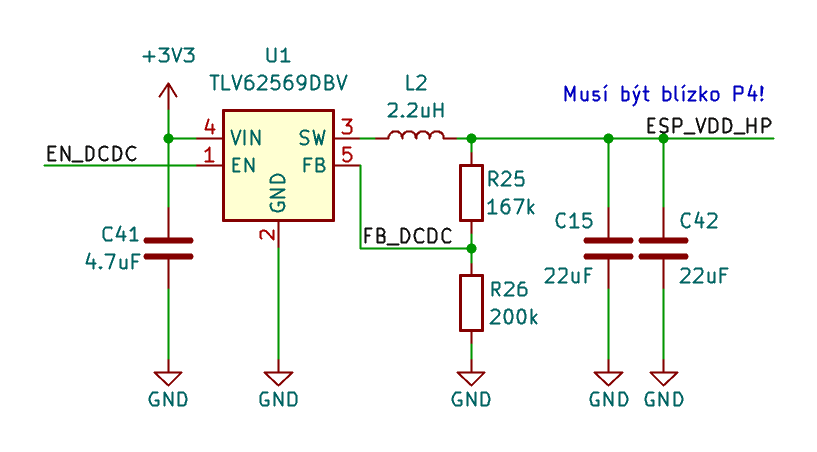
\includegraphics[width=0.7\linewidth]{pictures/hpbuck.png}
    \caption{Schména zapojení měniče pro napájení HP pinů \textit{[Zdroj: Vlastní]}}
    \label{fig:hpbuck}
\end{figure}
Programování zařízení je v tomto projektu navrženo pouze přes USB. Mikrokontrolér sice obecně umožňuje i programování přes UART, tato možnost však v daném návrhu není využita. Pro vstup do programovacího režimu je osazeno tlačítko SW1, připojené k GPIO 35.  Strapping piny se čtou během bootování a určují spouštěcí režim MCU. Tlačítko S1 slouží k aktivaci Joint Download Boot módu pro nahrávání firmwaru — při jeho stisku během startu se MCU spustí v režimu, který umožňuje download nového kódu přes USB. Podrobněji jsou bootovací režimy a jejich konfigurace strapping pinů uvedeny v tabulce~\ref{tab:boot_modes}.

\begin{table}[h]
\centering
\begin{tabular}{|l|c|c|c|c|}
\hline
\textbf{Boot Mode} & \textbf{GPIO35} & \textbf{GPIO36} & \textbf{GPIO37} & \textbf{GPIO38} \\
\hline
SPI Boot mode (default)\textsuperscript{1} & 1 & x & x & x \\
\hline
Joint Download Boot mode\textsuperscript{2} & 0 & 1 & x & x \\
\hline
SPI Download Boot mode\textsuperscript{3} & 0 & 0 & 0 & 1 \\
\hline
Invalid Combination\textsuperscript{4} & 0 & 0 & 0 & 0 \\
\hline
\end{tabular}
\caption{BOOT režimy dle kombinace strapping pinů ESP32-P4 \textit{[Zdroj: \cite{esp32p4_trm}]}}
\label{tab:boot_modes}
\end{table}
\begin{figure}
    \centering
    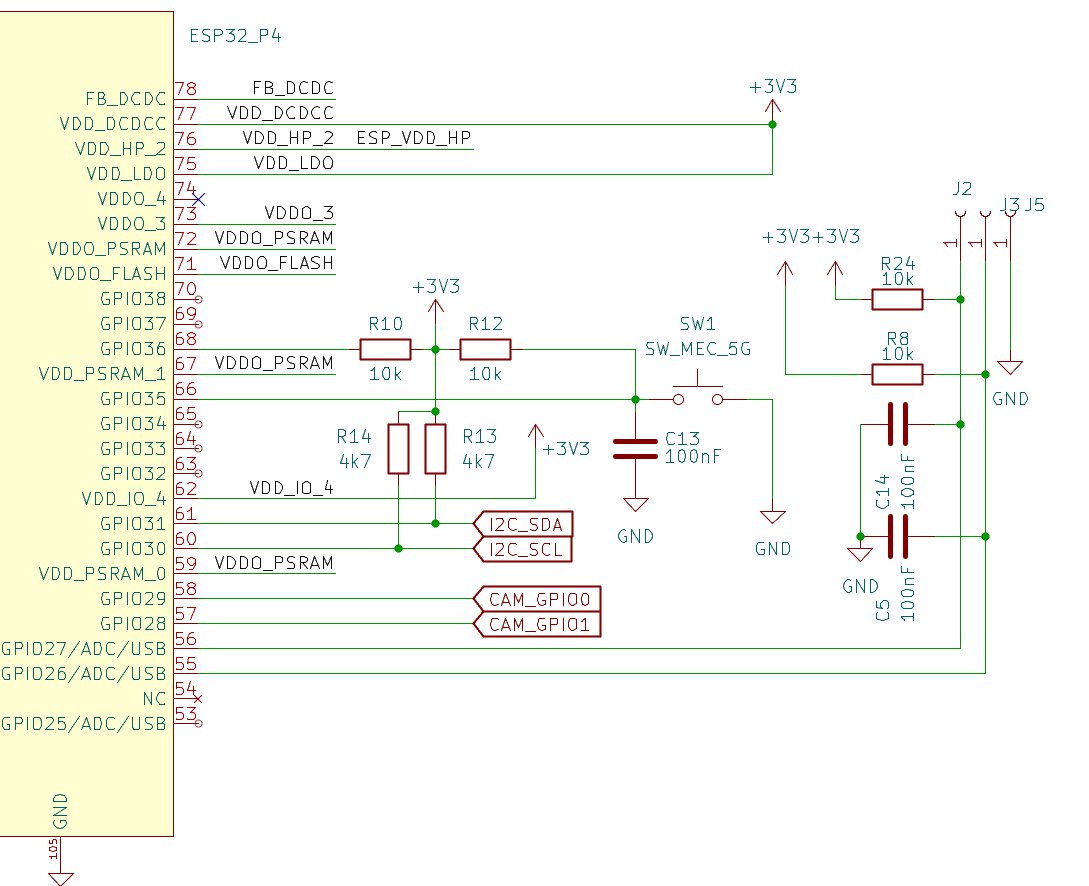
\includegraphics[width=0.8\linewidth]{pictures/i2c_bootstrappy_.png}
    \caption{Zapojení kolem ESP32-P4 popsané v této sekci: I2C pull-upy, reset a startovací vazby. \textit{[Zdroj: Vlastní]}}
    \label{fig:i2c_bootstrappy}
\end{figure}

Na obrázku~\ref{fig:i2c_bootstrappy} je zachycena pravá část MCU, kde se nachází BOOT strapping piny (GPIO 35--38)~\cite{esp32p4_trm}, interní regulátor pro napájení Flash a SRAM pamětí (\texttt{VDD\_LDO}).

Dále je na obrázku~\ref{fig:i2c_bootstrappy} zachyceno I2C rozhraní, připojené k pinům GPIO 30 a 31. Kvůli designu samotné sběrnice, kde zařízení pouze „tahá"~napětí na logickou nulu, jsou zde osazeny pull-up rezistory \texttt{R14} a \texttt{R15} (oba 4,7 k$\Omega$).


\subsection{Externí krystal}
Hodinový systém je doplněn externím 40MHz krystalem a dvojicí zátěžových kondenzátorů podle doporučení výrobce\cite{local_kicad,esp32p4_ds}. Tato část má přímý vliv na stabilní start systému i na přesnost časování vysokorychlostních periferií. Bez tohoto krystalu by kamera nemohla spolehlivě fungovat, protože by nebylo možné zajistit stabilní taktování pro zpracování obrazových dat.
\begin{figure}
    \centering
    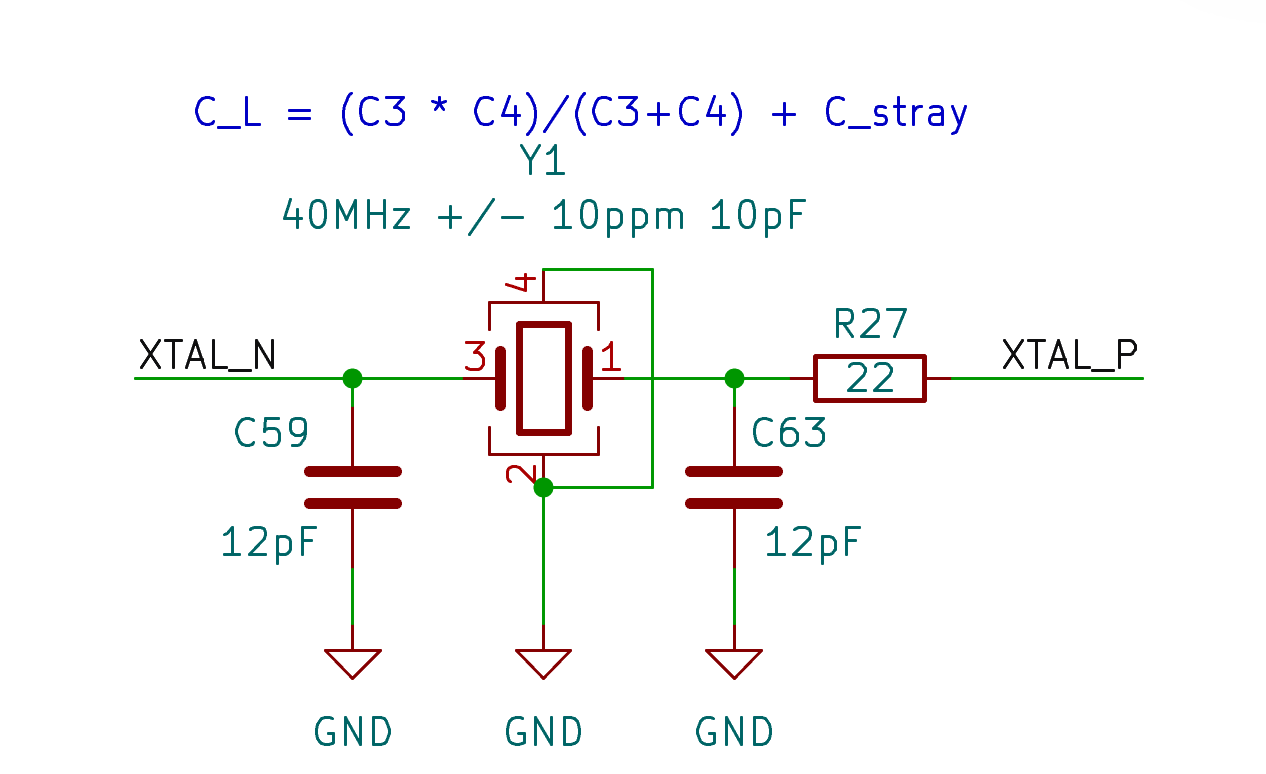
\includegraphics[width=0.7\linewidth]{pictures/xtal.png}
    \caption{Zapojení externího krystalu v eschématu. \textit{[Zdroj: Vlastní]}}
    \label{fig:xtal}
\end{figure}
Na obrázku~\ref{fig:xtal} je znázorněno zapojení 40MHz krystalu Y1 a jeho podpůrných součástek. Kondenzátory C59 a C63 mají hodnotu 12 pF anastavují správnou zátěž a stabilitu oscilátoru. Sériový odpor R27 o hodnotě 22~$\Omega$ slouží k tlumení kmitů a pomáhá omezit rušení.
Krysatal by měl výt osazen ve vzdálenosti alespoň 4,5 mm od MCU\cite{esp32p4_trm}, aby se zabránilo rušení.

Podrobnější informace o doporučeném zapojení napájecích domén a startovacích podmínkách uvádí datasheet a technický referenční manuál výrobce\cite{esp32p4_trm,esp32p4_ds}.


\section{Napájení periférií}
Napájecí část je navržena pro provoz z jednoho akumulátoru 7,2 V a je rozdělena do několika samostatných větví podle typu zátěže\cite{local_readme}. Ve schématu jsou osazeny měniče CONV1 (\texttt{AP63203WU}, pevný výstup 3,3 V), CONV2 (\texttt{AP63200WU}, nastavený na 5,5 V pro komunikaci s objektivem) a CONV4 (\texttt{AP63200WU}, nastavený na 6 V pro obsluhu servo motorů v objektivu)\cite{ap63200,local_kicad}.

Měnič CONV1 s obvodem \texttt{AP63203WU} vytváří hlavní větev 3,3 V. Na jeho vstupu jsou oddělovací diody D1 a D4, které umožňují napájení jak z větve +7V2 z akumulátoru, tak z USB +5V. Na vstupu jsou také kondenzátory C6 (100 nF) a C7 (10 $\mu$F), na výstupu pak C9 a C10 (oba 22 $\mu$F), tlumivka L1 (3,9 $\mu$H), bootstrap kondenzátor C8 (100 nF) a zenerova dioda D6 (3,6 V). Toto řešení je uvedeno na obrázku~\ref{fig:3v3cascade}. Díky němu může zařízení v omezeném režimu běžet i pouze z USB, ale bez napájení a bez komunikace objektivu nebude dostupné nastavování clony ani autofocus.

Měnič CONV2 s obvodem \texttt{AP63200WU} je nastaven na výstup 5,5 V pro napájení logiky objektivu. Na vstupu jsou kondenzátory C43 (100 nF) a C44 (10 $\mu$F), na výstupu tlumivka L3 (10 $\mu$H), kondenzátory C46 a C47 (oba 22 $\mu$F), bootstrap kondenzátor C45 (100 nF) a zenerova dioda D2 (5,7 V). Rezistory pro nastavení výstupního napětí jsou vybrány podle rovnice~\ref{nastavenimenice} poskytnuté výrobcem:
\begin{equation}
R_{1} = R_{2} \cdot \left(\frac{V_{OUT}}{0.8V}-1 \right)
\label{nastavenimenice}
\end{equation}
Toto zapojení je zachyceno na obrázku~\ref{fig:lenslogic}.

Měnič CONV4 (AP63200WU) je v zapojení použit jako samostatná větev pro napájení hlavních pohonů v objektivu, s výstupním napětím cca 6 V. Na vstupu (síť +7V2) jsou kondenzátory C48 (100 nF) a C49 (10 $\mu$F) pro odrušení; spínací stupeň používá bootstrap kondenzátor C50 (100 nF) a za ním následuje tlumivka L4 (10 $\mu$H). Výstupní filtrace tvoří kondenzátory C51 a C52 (oba 22 $\mu$F). Nastavení výstupního napětí realizuje dělič R7/R6 (R7 = 100 k$\Omega$ na výstupu, R6 = 16 k$\Omega$ k zemi) osazený podle rovnice \ref{nastavenimenice}, čímž se dosahuje cílové hodnoty~6 V. Pro finální vyhlazení je zapojena zenerova dioda D3 (6,2 V). Toto zapojení je zobrazeno na obrázku~\ref{fig:lensmainpower}.
\begin{figure}
    \centering
    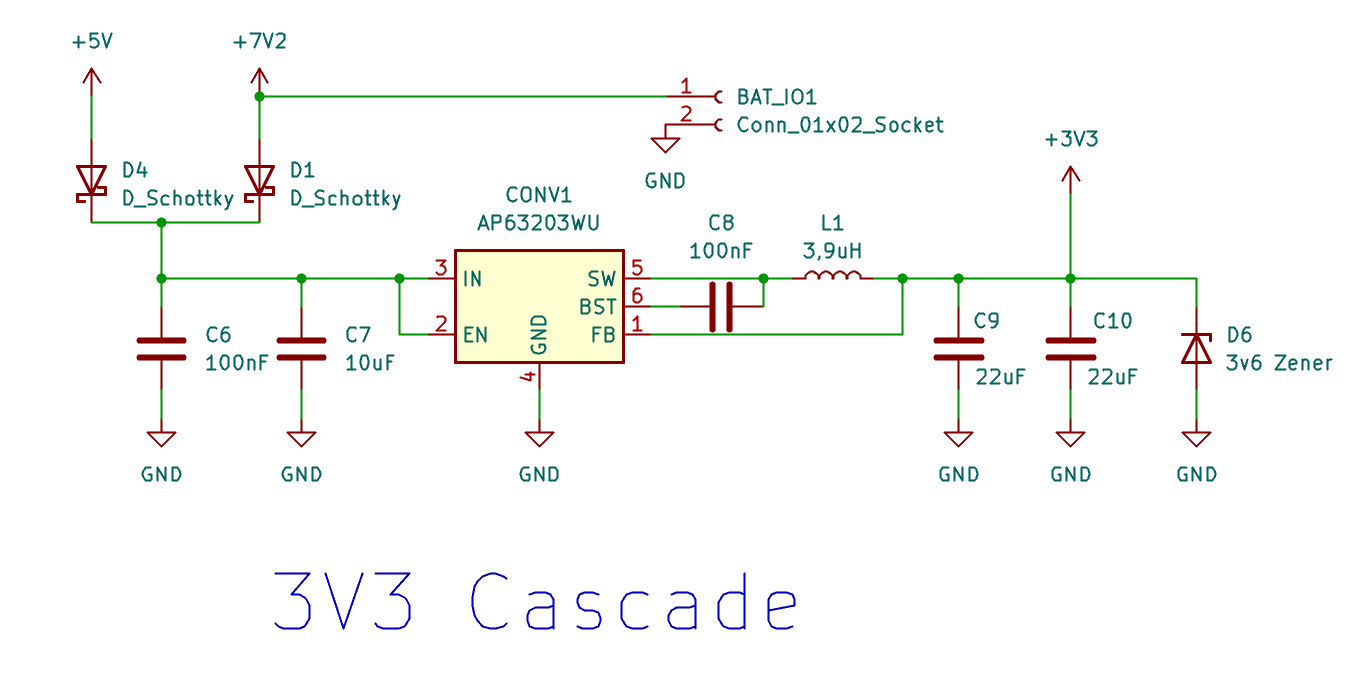
\includegraphics[width=1\linewidth]{pictures/3V3cascade.png}
    \caption{Měnič na 3,3 V v eschématu \textit{[Zdroj: Vlastní]}}
    \label{fig:3v3cascade}
\end{figure}
\begin{figure}
    \centering
    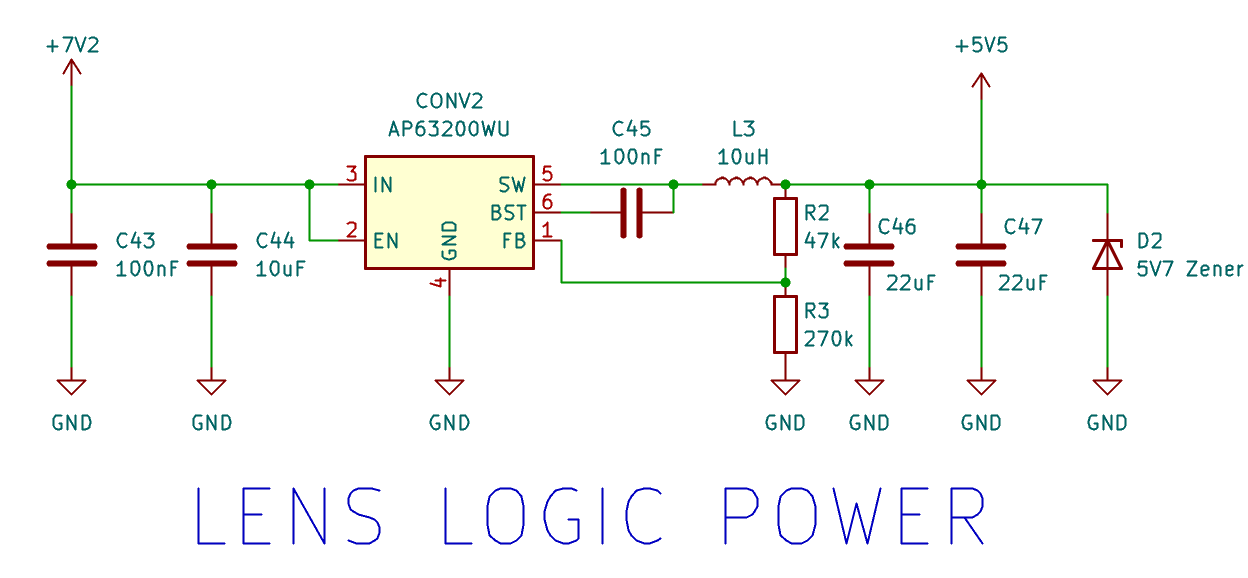
\includegraphics[width=1\linewidth]{pictures/lenslogicpower.png}
    \caption{Zapojení měniče napětí pro komunikaci s objektivem \textit{[Zdroj: Vlastní]}}
    \label{fig:lenslogic}
\end{figure}
\begin{figure}
    \centering
    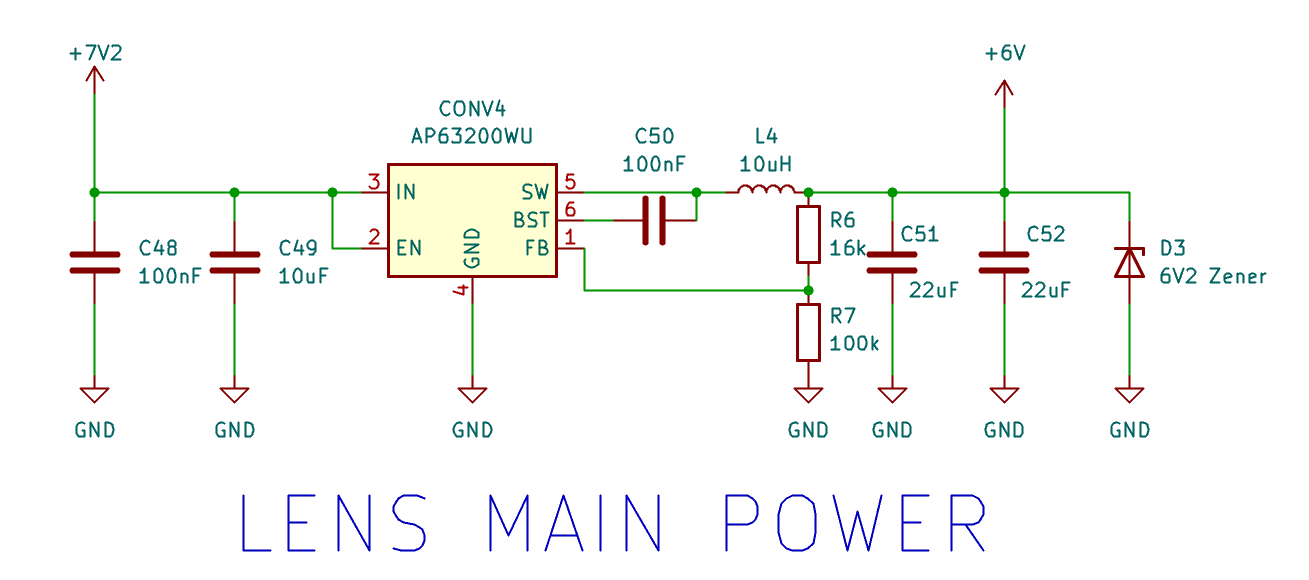
\includegraphics[width=1\linewidth]{pictures/lensmainpower.png}
    \caption{Zapojení měniče napětí pro obsluhu servo motorů v objektivu \textit{[Zdroj: Vlastní]}}
    \label{fig:lensmainpower}
\end{figure}
\section{Externí Flash paměť}

Externí flash paměť je osazena jako samostatný nevolatilní prostor pro firmware a provozní data\cite{w25q256,local_kicad}. Připojení je řešeno přes QSPI, aby byla zajištěna dostatečná propustnost při startu systému i při běhu aplikace.

Ve schématu je osazena paměť ESP\_FLASH1 typu \texttt{W25Q256JVEIQ}. Stabilitu této části zajišťuje zejména důraz na velmi nízké odchylky mezi jednotlivými cestami. To je důležité zejména kvůli vysokým přenosovým rychlostem. Schéma zapojení a n8vrh routování této části jsou zobrazeny na obrázku~\ref{fig:flash}. Všimněte si, že všechny cesty jsou vedeny v jedné vrstvě, jsou co nejkratší a mají stejné délky vyladěné pomocí tzv. „meandrů“ . Díky tomu je minimalizováno riziko ztráty dat kvůli rušení nebo odrazům signálu.
\begin{figure}
    \centering
    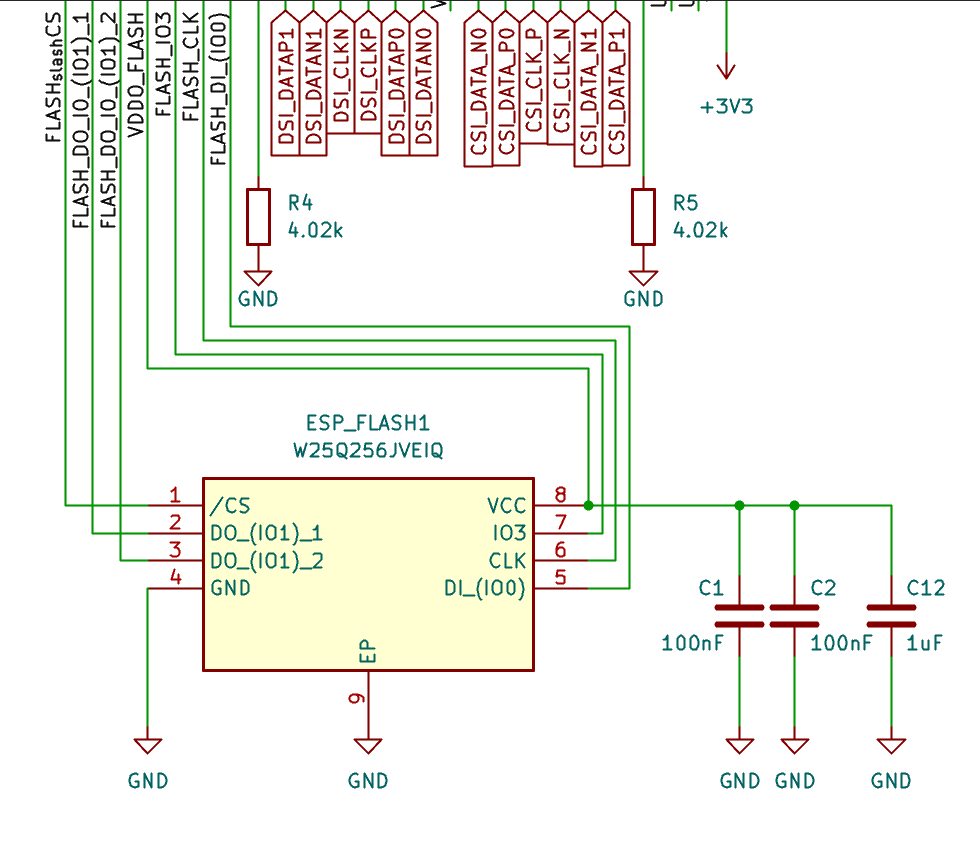
\includegraphics[width=0.7\linewidth]{pictures/flash.png}
    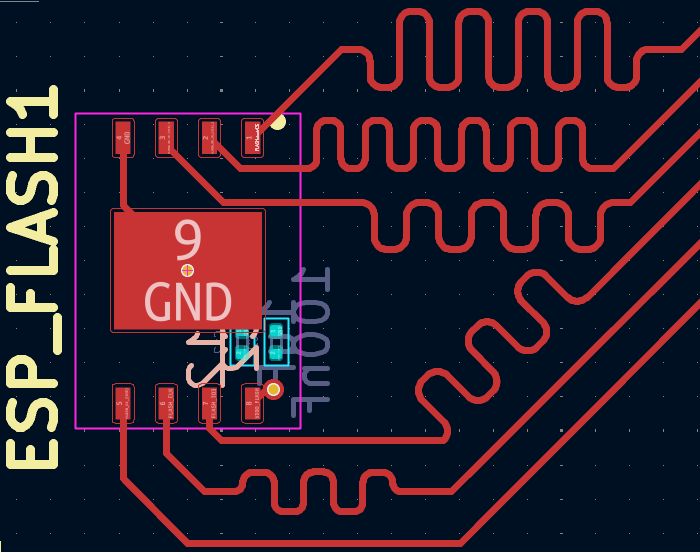
\includegraphics[width=0.7\linewidth]{pictures/flashpcb.png}
    \caption{Zapojení externí flash paměti v eschématu a v PCB editoru. \textit{[Zdroj: Vlastní]}}
    \label{fig:flash}
\end{figure}

\section{Konektory pro připojení periférií}
\subsection{Konektor pro zapojení kamerového modulu}
Kamerový modul je připojen přes 15pinový FFC konektor. Vedeny jsou diferenciální páry MIPI CSI, řídicí sběrnice I2C, napájení a řídicí signály pro zapnutí modulu. Stejně jako u Flash paměti je důležité dbát na symetrii délek cest a jejich tvar pro zabránění rušení.
\begin{figure}
    \centering
    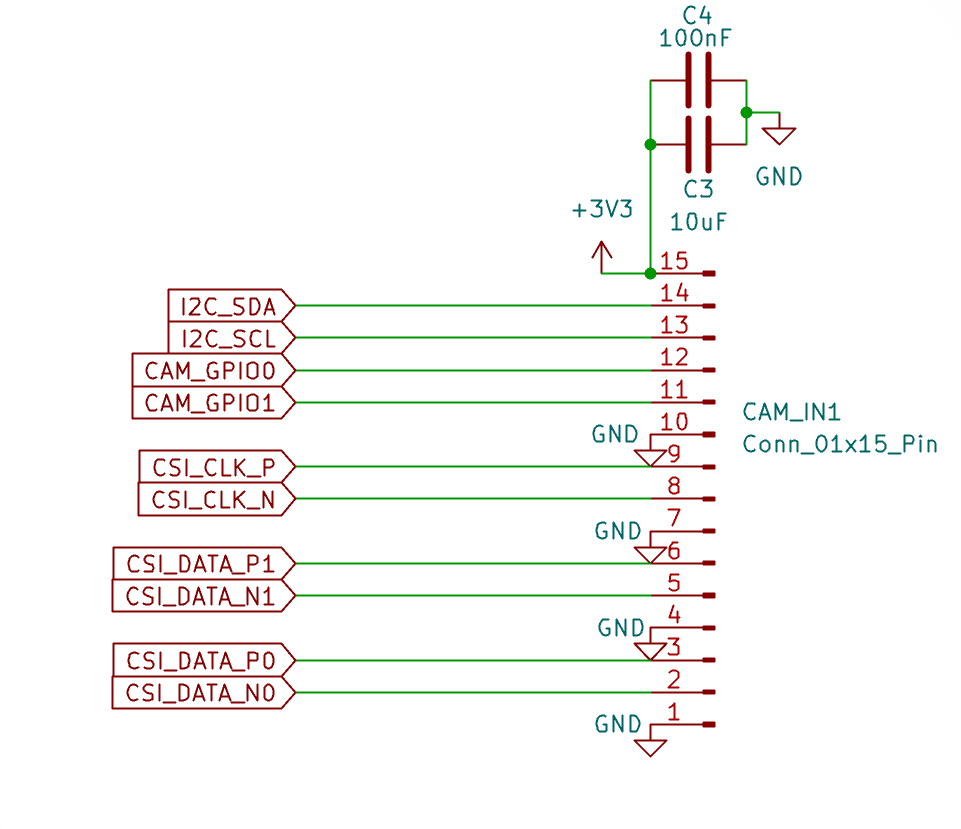
\includegraphics[width=0.7\linewidth]{pictures/kamera.png}
    \caption{Zapojení konektoru pro připojení kamerového modulu \texttt{IMX219}. \textit{[Zdroj: Vlastní]}}
\end{figure}

Text této části je záměrně veden obecně na úrovni použitého rozhraní a zapojení. Konkrétní parametry obrazového snímače je vždy nutné vztáhnout k reálně osazenému kamerovému modulu. Je tedy možné použít kamerový modul se stejným pinoutem, ale s jinými parametry, a to i bez nutnosti úprav v zapojení. Naopak použití modulu s jiným pinoutem by vyžadovalo zásadní úpravy v zapojení i v softwaru.

\subsection{Konektor pro zapojení displaye}
Displej je připojen přes samostatný 15pinový FFC konektor. Na tomto rozhraní jsou vyvedeny MIPI DSI páry pro obrazová data a pomocné signály I2C pro obsluhu dotykové vrstvy\cite{local_kicad,waveshare}.
\begin{figure}
    \centering
    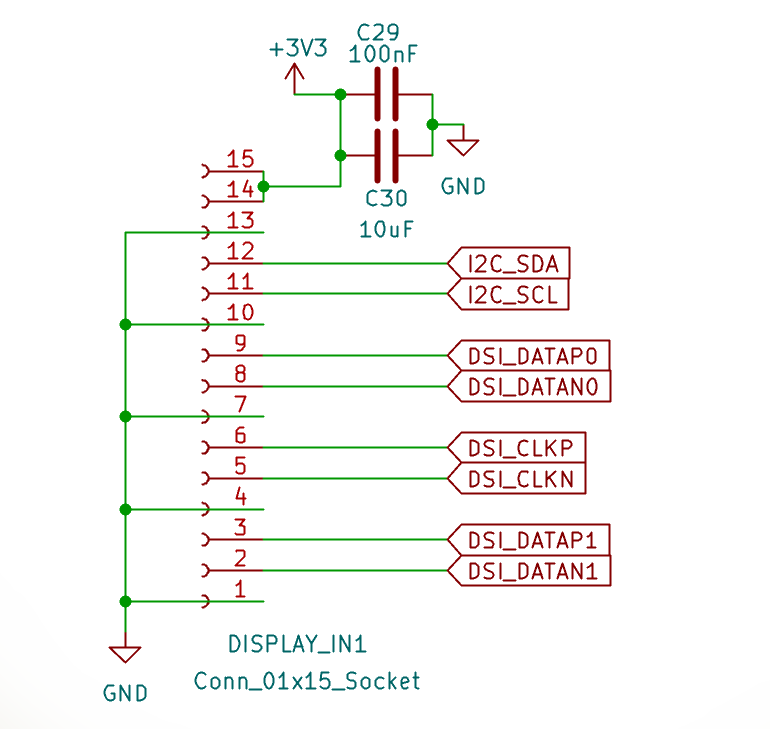
\includegraphics[width=0.7\linewidth]{pictures/display.png}
    \caption{Zapojení konektoru pro připojení displeje v eschématu. \textit{[Zdroj: Vlastní]}}
\end{figure}

I zde je nutné dbát na délkovou symetrii cest a jejich tvar, aby se minimalizovalo rušení a ztráta dat při přenosu obrazových informací.
\begin{figure}
    \centering
    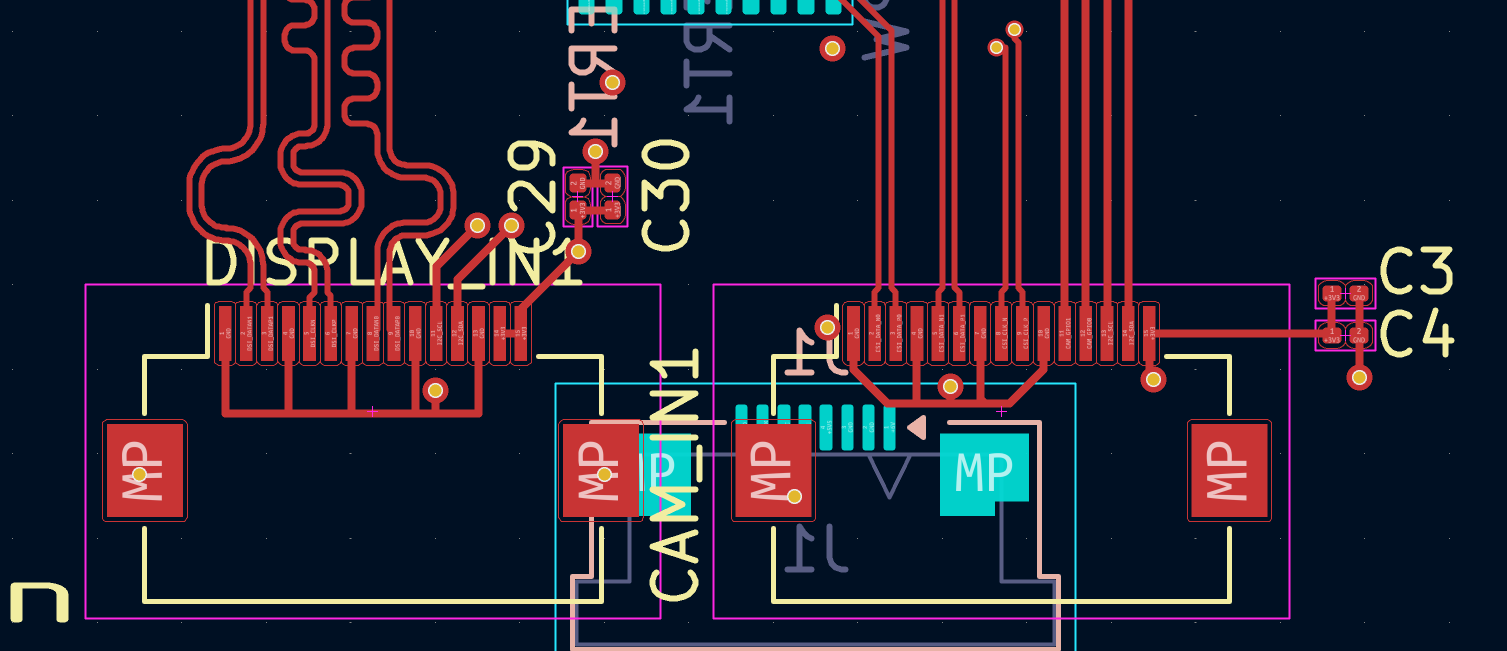
\includegraphics[width=\linewidth]{pictures/pcbdsiacam.png}
    \caption{Návrh pro zapojení konektoru pro připojení kamery (vlevo) a displaye (vpravo). \textit{[Zdroj: Vlastní]}}
\end{figure}
\subsection{Dock pro umístění SD karty}
Pro ukládání snímků je osazen konektor pro MicroSD kartu\cite{local_kicad}. Kromě datových linek je využita i detekce vložení karty, což zjednodušuje obsluhu v softwaru a snižuje riziko zápisu na neosazené médium.
\begin{figure}
    \centering
    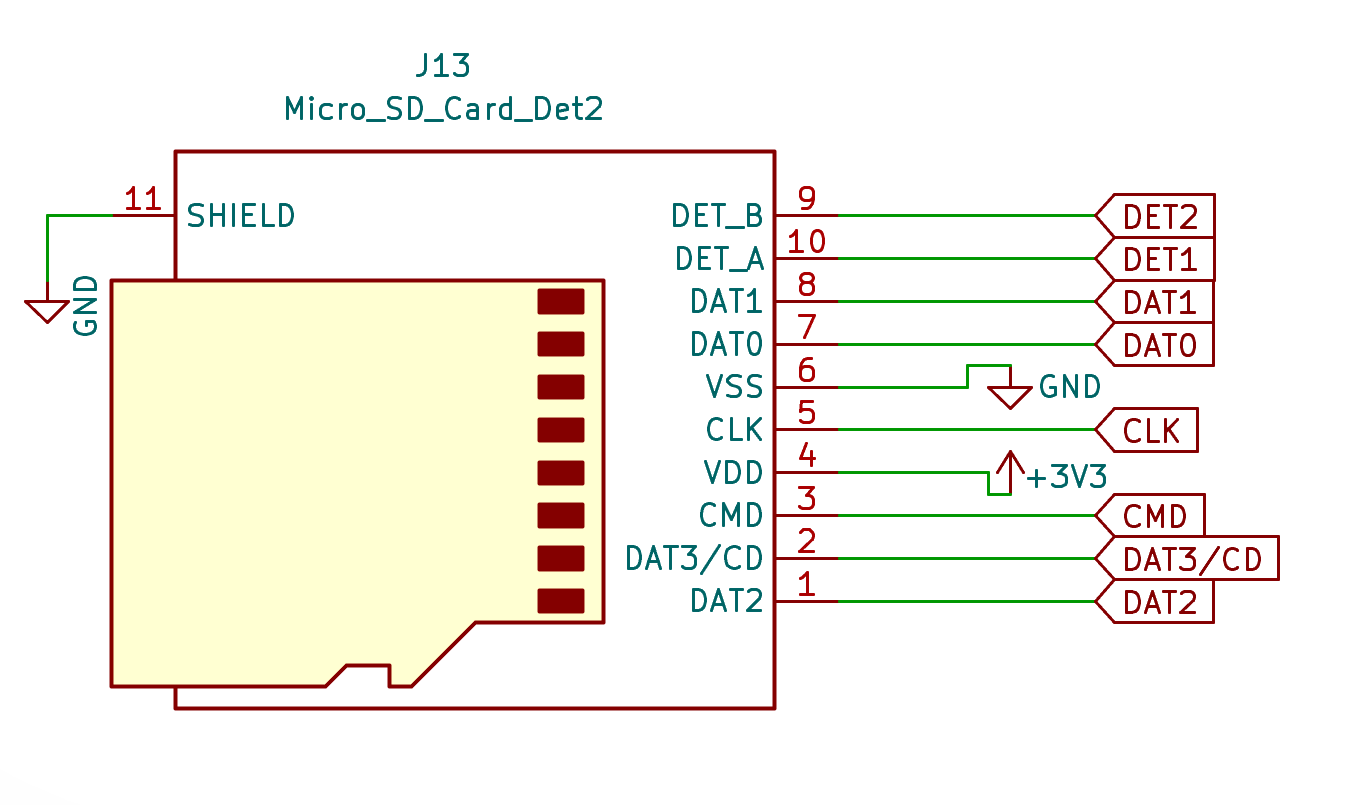
\includegraphics[width=0.5\linewidth]{pictures/sdkarta.png}
    \caption{Zapojení slotu pro SD kartu v eschématu. \textit{[Zdroj: Vlastní]}}
\end{figure}
\subsection{Konektory pro tlačítka ovládání}
\begin{figure}
    \centering
    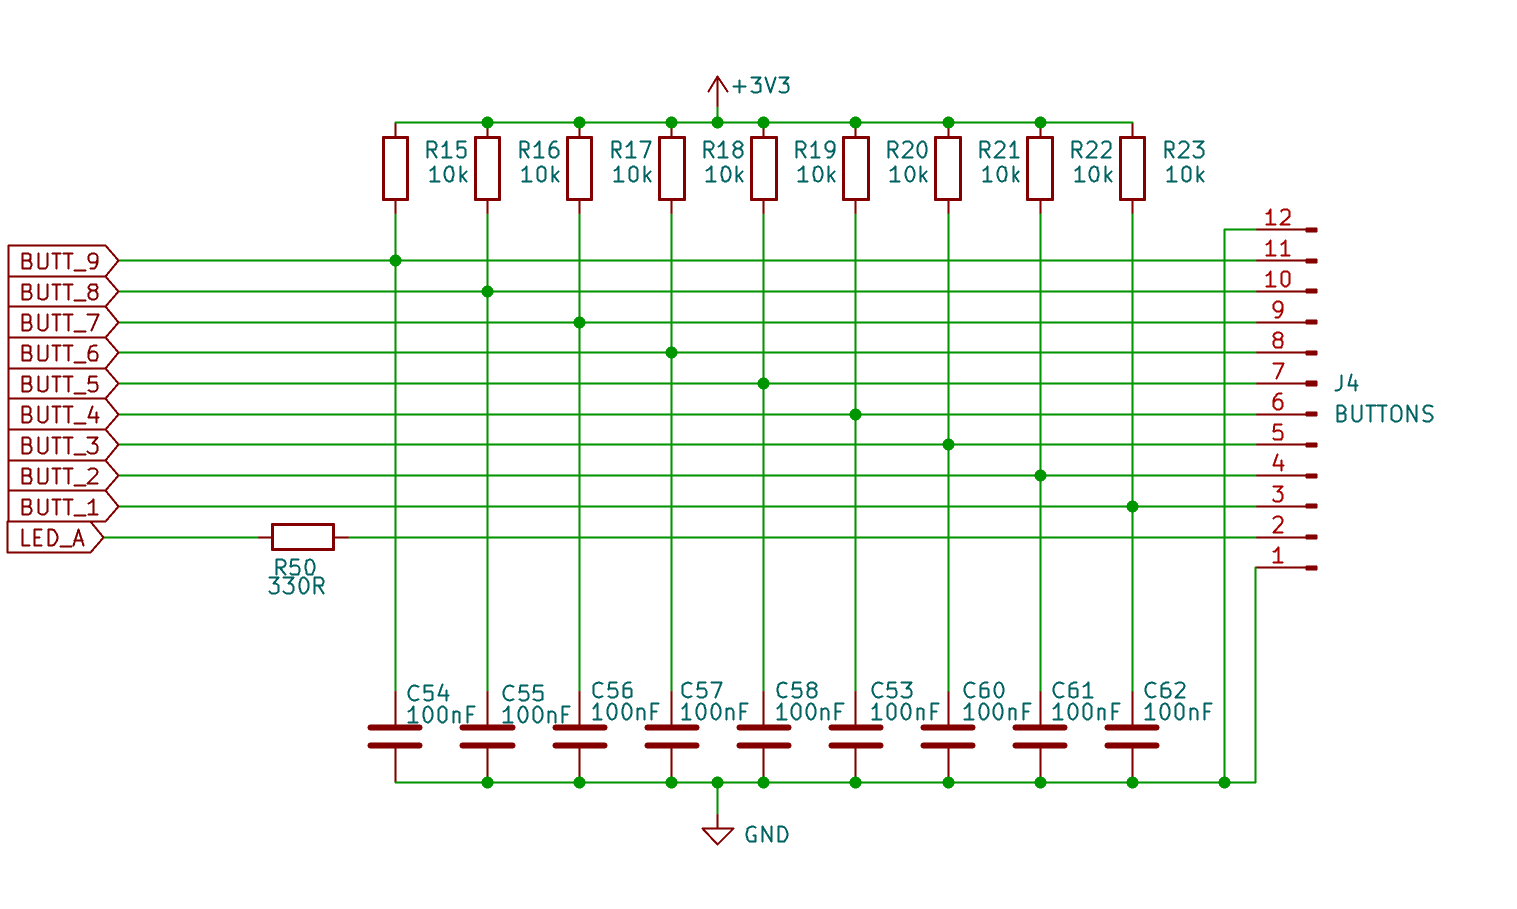
\includegraphics[width=\linewidth]{pictures/tlacitka_550D.png}
    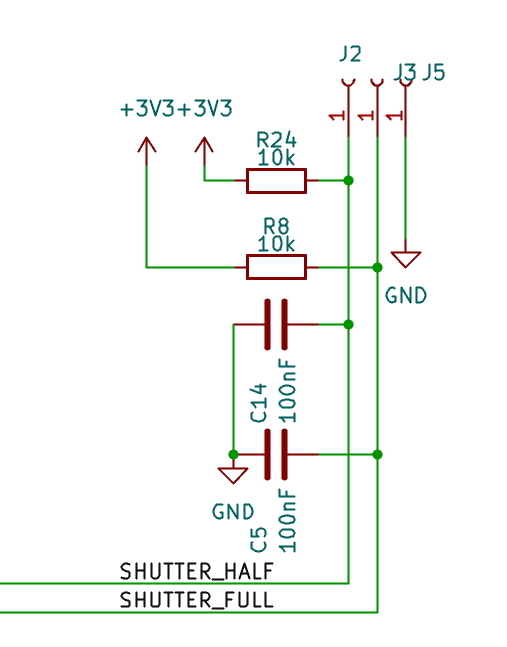
\includegraphics[width=0.5\linewidth]{pictures/spoust.png}
    \caption{Zapojení konektorů pro připojení ovládacích tlačítek v eschématu. Nahoře hlavní olvádací rozhraní, dole tlačítka spouště Fotaoparátu. \textit{[Zdroj: Vlastní]}}
\end{figure}

Pro připojení ovládacích tlačítek jsou navrženy dva konektory, které umožňují připojení jak hlavního ovládacího rozhraní (pro nastavení parametrů a navigaci v menu), tak i samostatného tlačítka spouště. Ovládací tlačítka, a k tomu indikační červená led dioda, jsou připojena k GPIO 42--52. Celá tato deska byla recyklována z rozbraného modelového fotoaparátu Canon 550D. Tlačíko spouště je stejného původu, ale je připojeno samostatně kvůli své specifické funkci a umístění v konstrukci zařízení. Kvůli komplikovanému zapojení na původní desce 550D je nutné připojit tlačítko spouště samostatně na plošném spoji vlastní výroby, proto je na návrhu osazen samostatný konektor pro tento účel.

\section{Převodník logických úrovní pro komunikaci s objektivem}
Pro komunikaci s objektivem Canon EF je osazen obousměrný převodník logických úrovní \texttt{TXS0108EPW}\cite{txs0108e,canon_ef_notes}. Důvodem je rozdíl mezi logikou mikrokontroléru a úrovněmi na straně objektivu.
\begin{figure}
    \centering
    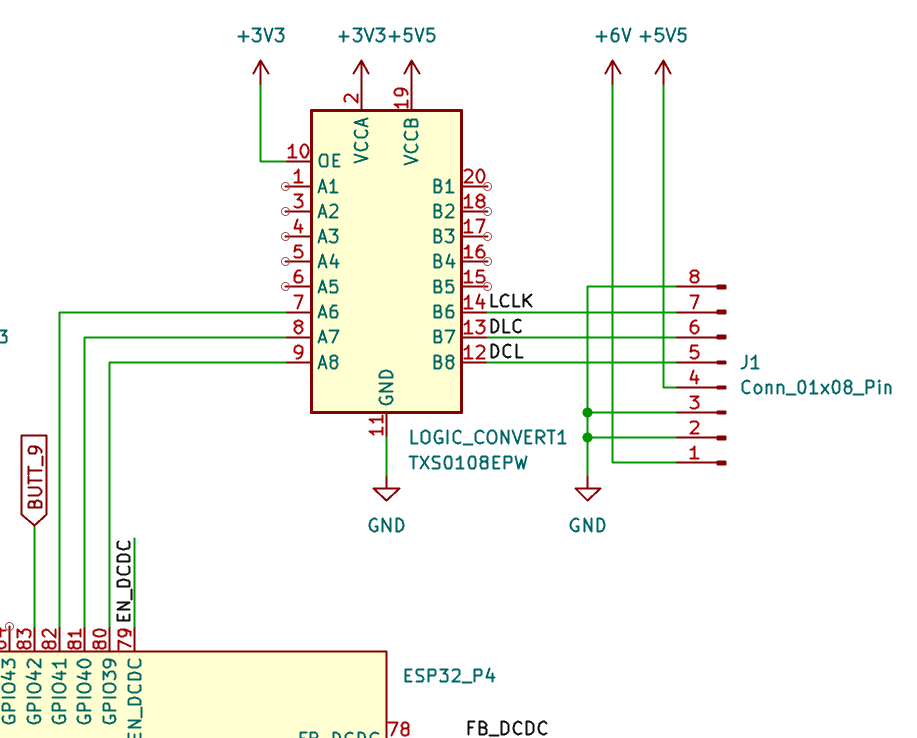
\includegraphics[width=0.7\linewidth]{pictures/prevodniklogurovni.png}
    \caption{Zapojení převodníku logických úrovní pro komunikaci s objektivem v eschématu. \textit{[Zdroj: Vlastní]}}   
\end{figure}

Z dostupných měření vyplývá, že část EF signálů není spolehlivá při 3,3V úrovni, proto je oddělení napěťových domén v této části nezbytné\cite{canon_ef_notes,magic_lantern}.

\section{USB-C USB 2.0 konektor}
Datové a servisní rozhraní je řešeno přes USB-C v režimu USB 2.0\cite{local_kicad,usb_typec}. Rozhraní slouží pro programování firmwaru, ladění i napájení během vývoje.

Na CC pinech jsou osazeny pull-down rezistory (Rd) pro indikaci zařízení; v našem návrhu jsou to R9 a R1 (5.1~k$\Omega$) k zemi, což signalizuje hostu, že jde o device. Datové linky D$+$ a D$-$ jsou chráněny ESD/TVS součástí (\texttt{ESDA6V1U1RL}) a mohou být vedeny přes common-mode choke pro lepší EMI/EMC potlačení. SBU piny nejsou v návrhu využity.

V kombinaci s nativní podporou USB v ESP32-P4 toto řešení výrazně zjednodušuje oživení i další vývoj\cite{esp32p4_ds,esp32p4_web}.

\begin{figure}
    \centering
    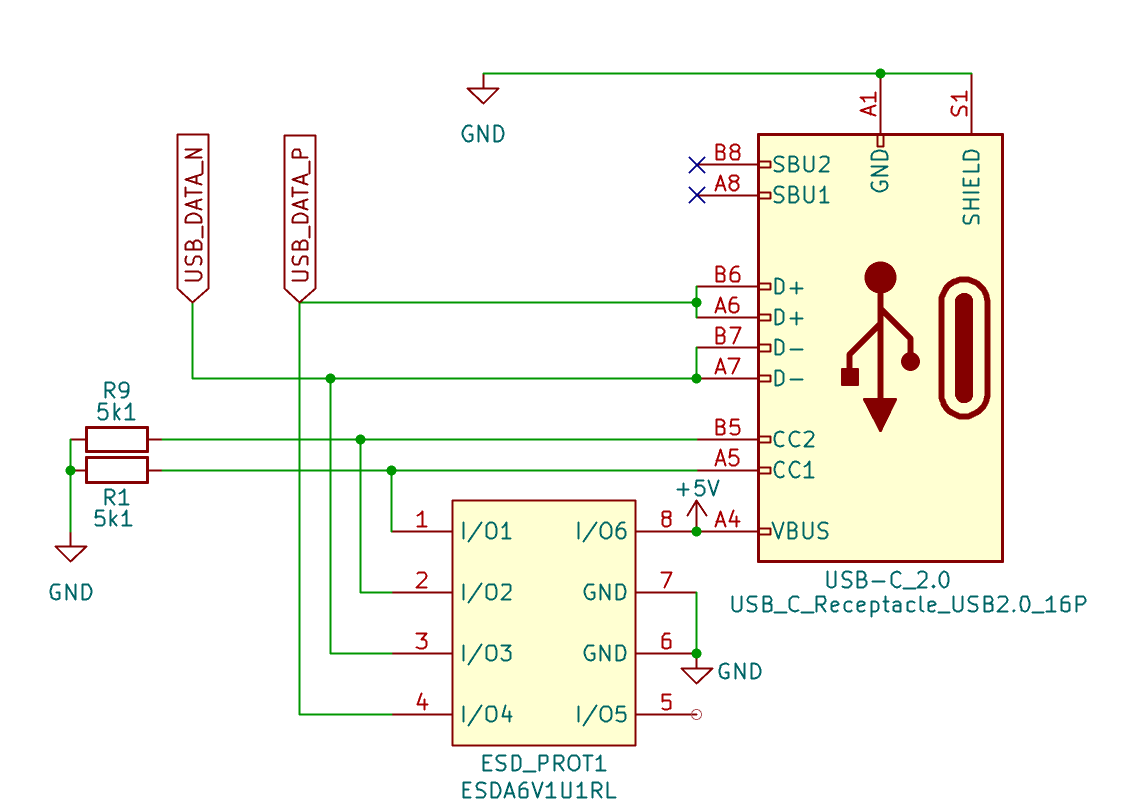
\includegraphics[width=0.7\linewidth]{pictures/usb-c.png}
    \caption{Zapojení USB-C konektoru v eschématu. \textit{[Zdroj: Vlastní]}}
\end{figure}

\chapter{Plánvané oživení a konstrukce}

% Poznámka o stavu
Praktické oživení hardwaru a dokončení mechanické konstrukce nebyly dokončeny do termínu uzávěrky, neboť jsem přecenil své síly a podcenil časový limit. Následující části proto popisují plánované kroky a doporučený postup pro systematické oživení a dokončení návrhu mechaniky.

\section{Plánované oživení}
Pro úspěšné softwarové oživení desky je třeba připravit konzistentní vývojové prostředí, automatizované nástroje pro flashování a sběr logů a repozitář s minimálním testovacím firmwarem. V praxi to znamená nastavit toolchain a build systém (např. ESP‑IDF nebo jiný zvolený framework) a zajistit stabilní verze kompilátorů a utilit, připravit skripty pro pohodlné flashování přes USB a zachytávání sériového výstupu (UART/USB logging) a mít v repozitáři konfiguraci buildu spolu s jednoduchým testovacím obrazem (např. minimal boot image nebo „blinky“) pro rychlé ověření hardwaru.
Po této přípravě následuje vlastní sekvence bring‑upu: nejprve se nahraje bootloader a velmi jednoduchý firmware, který pouze inicializuje periférie a posílá základní diagnostické zprávy přes sériovou linku. Na základě těchto logů ověříme boot sekvenci, přítomnost a verze paměti a dosažitelnost důležitých pinů. Dále firmware krokově rozšiřujeme o inicializaci hodinového systému a QSPI rozhraní tak, aby bylo možné korektně číst z externí flash paměti.

Následují kroky zaměřené na periferie vyšší úrovně: přidání a otestování ovladače SD karty a připojení souborového systému (např. FAT) s ověřením čtení a zápisu souborů, integrace ovladače displeje s jednoduchým vykreslením testovacího obrazu a následně integrace ovladače kamery/CSI — nejprve přes I2C inicializovat senzor a poté spustit jednoduchý capture, uložit snímek do paměti a ověřit jeho zápis na SD nebo přenos přes USB.

Během celého procesu je vhodné zavést jednoduchou diagnostiku ve firmwaru (watchdog, zdravotní telemetrie, detekce chyb) a zajistit možnost bezpečného aktualizačního mechanismu (OTA nebo flash přes USB) pro případ rychlých oprav. Pro opakované ověření se připraví automatizované testovací skripty: smoke test pro boot a základní I/O, sady testů pro QSPI/SD/I2C a funkční scénáře zahrnující pořízení snímku a jeho zobrazení či uložení.

Do ověřovacích metrik softwarového oživení patří především úspěšný boot bez kritických chyb, schopnost číst a zapisovat do externí paměti a SD karty, stabilita karetní a kamerové komunikace (latence a propustnost) a spolehlivost aktualizačního procesu. Tyto body by měly být zachyceny v jednoduchých testovacích protokolech, které umožní opakovat ověření i po případných hardwarových úpravách.

\section{Plánovaná konstrukce}
Z důvodu komplexity mechanické konstrukce bajonetu, který bych sám nemohl udělat pro bezpečné uchycení objektivu, jsem se rozhodl využít tělo a vybrané periferie z modelu Canon 550D. Toto řešeení jsem si vybral jako spíše dočasné, jelikož by umožnilo rychlejší vývoj a oživení. V budoucnu bych rád navrhl vlastní mechanickou konstrukci, jelikož je potřeba brát v úvahu i tzv. flange, neboli vzdálenost mezi bajonetem a snímačem, která je u Canon EF 44 mm. Proto mám v plánu vytořit vlastní tělo Fotaoparátu, s vnořeným bajonetem EF.

\chapter{Závěr}
Bohužel jsem neodhadl dobu pro pečlivé kontrování, a lehce přecenil své schopnosti z hlediska elektrotechniky. To způsobilo to, že jsem se nedostal do fáze oživení a testování, což je pro mě velkou škodou.

Práce v KiCADu není zcela skončená, návrh plošného spoje se stal zmatečným kvůli častému předělávání nákreu, když jsem našel chybu v zapojení, které v mé hlavě bylo velmi jednoduché. Živoucím příkladem je zapojení měničů napětí, protože jsem se snažil navrhnout co nejjednodušší řešení, abych posléze zjstil že v datasheetu je ukázka zapojení, kde byly i další součástky pro stabilizaci a odrušení, což vedlo k tomu, že jsem musel předělat celý návrh napájecí části.
Schéma je na tom lépe, hlavně kvůli ochotě pana učitele Švihly, který se mi ve svém limitovaném čase snažil pomáhat.

Mám v plánu pokračovat v práci i přístí rok a dokočit co jsem začal.
% CIATCE ---------------------------------------------------------------------------
\begin{thebibliography}{99}
\addcontentsline{toc}{chapter}{Literatura}

% \bibiintem{reference} referenci pak pouzijte v textu \cite{reference}.
% dodržujte formátování citací dle normy: Jméno, název (kurzívou), vydavatel, rok, ...
% Pořadí citací podle výskytu v textu. 

\bibitem{ap63200} DIODES INCORPORATED. \textit{AP63200/AP63201/AP63203/AP63205 -- Buck Converter Datasheet}. Dostupné z: \url{https://www.diodes.com/assets/Datasheets/AP63200-AP63201-AP63203-AP63205.pdf}. [cit. 2026-04-23].

\bibitem{local_kicad} HOVORKA, V. \textit{Projektové schéma v KiCadu (fotaoparát.kicad\_sch, power.kicad\_sch, peripherals.kicad\_sch)}. Lokální projektová dokumentace, 2026.

\bibitem{local_readme} HOVORKA, V. \textit{RP-Hovorka/readme.md -- hardware TODO a napájecí větve}. Lokální projektová dokumentace, 2026.

\bibitem{esp32p4_ds} ESPRESSIF SYSTEMS. \textit{ESP32-P4 Datasheet}. Lokální soubor: datasheeshty/Esp32-p4\_datasheet\_en.pdf, 2026.

\bibitem{esp32p4_trm} ESPRESSIF SYSTEMS. \textit{ESP32-P4 Technical Reference Manual}. Lokální soubor: datasheeshty/Esp32-p4\_technical\_reference\_manual\_en.pdf, 2026.

\bibitem{w25q256} WINBOND. \textit{W25Q256JV -- Serial NOR Flash Datasheet}. Lokální soubor: datasheeshty/w25q256jv dtr revc 10252016.pdf, 2016.

\bibitem{arducam_shop} RPI SHOP CZ. \textit{Arducam IMX219 8 MPx kamerový modul}. Dostupné z: \url{https://rpishop.cz/635962/arducam-imx219-8-mpx-kamerovy-modul-s-objektivem-m12-ls1820-noir/}. [cit. 2026-04-23].

\bibitem{waveshare} WAVESHARE. \textit{2.8inch DSI LCD -- Product Page}. Dostupné z: \url{https://www.waveshare.com/product/displays/2.8inch-dsi-lcd.htm}. [cit. 2026-04-23].

\bibitem{waveshare_wiki} WAVESHARE. \textit{2.8inch\_DSI\_LCD -- Wiki}. Dostupné z: \url{https://www.waveshare.com/wiki/2.8inch_DSI_LCD}. [cit. 2026-04-23].

\bibitem{hirose_dm3} HIROSE ELECTRIC. \textit{DM3 Series -- MicroSD Card Connector Catalog}. Dostupné z: \url{https://www.hirose.com/en/product/document?clcode=&productname=&series=DM3&documenttype=Catalog&lang=en&documentid=D49662_en}. [cit. 2026-04-23].

\bibitem{esda6v1} STMICROELECTRONICS. \textit{ESDA6V1U1RL -- ESD Protection Device}. Dostupné z: \url{https://lcsc.com/product-detail/Diodes-ESD_STMicroelectronics_ESDA6V1U1RL_ESDA6V1U1RL_C118278.html}. [cit. 2026-04-23].

\bibitem{txs0108e} TEXAS INSTRUMENTS. \textit{TXS0108E -- 8-Bit Bidirectional Voltage-Level Translator}. Dostupné z: \url{https://www.ti.com/lit/ds/symlink/txs0108e.pdf}. [cit. 2026-04-23].

\bibitem{canon_ef_notes} HECTOR, M. \textit{software/canon-ef-protocol-notes.md}. Dostupné z: \url{https://gist.github.com/marcan/858c242db2fc595da1e0bb70a05192fc#file-canon-ef-protocol-notes-md} (reverse engineering EF sběrnice), 2026.

\bibitem{magic_lantern} MAGIC LANTERN TEAM. \textit{Magic Lantern}. Dostupné z: \url{https://www.magiclantern.fm}. [cit. 2026-04-23].

\bibitem{usb_typec} USB IMPLEMENTERS FORUM. \textit{USB Type-C Specification}. Dostupné z: \url{https://www.usb.org/sites/default/files/documents/usb_type-c.zip}. [cit. 2026-04-23].

\bibitem{esp32p4_web} ESPRESSIF SYSTEMS. \textit{ESP32-P4 Product Overview}. Dostupné z: \url{https://www.espressif.com/en/products/socs/esp32-p4}. [cit. 2026-04-23].


\end{thebibliography}
% konec citací

% Přílohy: 
\chapter*{Přílohy}
\pagenumbering{Roman}
\addcontentsline{toc}{chapter}{Přílohy}



\end{document}